\chapter{Calcolo Differenziale}

In questo capitolo sono trattate funzioni $f: A \mapsto \R^m$ con $A \subseteq \R^n$, dove $r,m \in \N$ e $n,m \geq 1$.\\
Generalmente, effetuata una dimostrazione per $m = 1$ è abbastanza semplice passare ad un $m > 1$ \textit{affiancando} le componenti, mentre non è altrettanto triviale il passaggio a $n > 1$.

\section{Preliminari}
In $\R^n$ verranno usate le (note) strutture vettoriale con la metrica Euclidea di \hyperref[ex:dist_eucl]{\cref*{ex:metriche} (\nameref*{ex:metriche})} % NOTE The \fullref command was not used on purpose to point this link straight to the right part of the aforementioned exercise

La base canonica di $R^n$ è indicata con $(e_1,\:\dotsc\:,e_n)$, $e_i$ è il vettore di $R^n$ con tutte le componenti nulle tranne la i-esima che vale 1. È dunque possibile scrivere un generico vettore $x$ si può quindi scrivere come combinazione lineare dei vettori della base canonica $x=\sum\limits_{i=1}^{n} x_i e_i$.

Nel caso $n=2$ è usata la notazione $(x,y)=xi+yj$. Nel caso $n=3$ è usata la notazione $(x,y,z)=xi+yj+zk$

Alcune classi di funzioni $f:A\subseteq\R^n\rightarrow\R^m$ hanno nomi particolari:
\begin{itemize}
	\item $n=1$,$m=1$: $f$ è una \textit{funzione reale di una variabile reale};
	\item $n=1$,$m>1$: $f$ è una \textit{curva} in $R^m$ (purché $f$ sia almeno continua e $A$ su un intervallo)
	\item $n>1$,$m=1$: $f$ è un \textit{campo scalare}
	\item $n>1$,$m>1$: $f$ è un \textit{campo vettoriale} (soprattutto nei casi $n=m=2$ e $n=m=3$)
\end{itemize}

\section{Derivate Parziali e Direzionali}
Direttamente dalla nozione di Analisi 1 di derivata, cioè
\begin{align*}
	f'(x_0) = \lim\limits_{t \to 0} \frac{f(x_0 + t) - f(x_0)}{t} \tag{\textbf{NB}. Analisi 1!}
\end{align*}
si estende il concetto di derivata alle funzioni in spazi $n$\textit{-dimensionali} mediante la seguente
\begin{definition}[Derivata Parziale e Direzionale]
	\label{def:deriv_direz}
	Sia $A \subseteq \R^n$, $f: A \mapsto \R^m$, $x_0 \in \circdot{A}$ e $v \in \R^n$ un vettore non nullo. Quando il limite
	\[\lim\limits_{t \to 0} \frac{(x_0 + tv) - f(x_0)}{t}\]
	esiste finito, il suo valore è la \textbf{Derivata Direzionale} di $f$ in $x_0$ nella direzione $v$ e si indica con $\boldsymbol{D_v f(x_0)}$
	\begin{note}
		\textbf{Non} è richiesto che la funzione sia \textbf{continua nello spazio} per calcolarne la derivata direzionale, è sufficiente sia continua nella direzione considerata. Vedasi \fullref{ex:deriv_solo_alcune_direz}
	\end{note}
	\begin{note}
		L'introduzione del vettore $v$ permette di eseguire un'operazione "sensata" in quanto sottrare uno scalare, come in Analisi 1, non avrebbe avuto significato per una funzione $f: A \mapsto \R^{\boldsymbol{m}}$.
	\end{note}

	Nel caso in cui $v = e_i$, allora $\boldsymbol{D_{e_i} f(x_0)}$ è la \textbf{Derivata Parziale $\boldsymbol{i}$\textit{-esima}}, che può anche essere indicata con $\boldsymbol{\frac{\partial f}{\partial x_i}(x_0)}$. Quindi le derivate parziali sono \textit{un caso particolare} delle derivate direzionali.\\

	\noindent Una funzione derivabile parzialmente in ogni direzione è detta \textbf{Derivabile}.

	\begin{note}
		Altre notazioni comunemente utilizzate per le derivate direzionali sono: $D_i f$, $D_{x_i} f$, $\partial_i f$, $\partial_{x_i} f$, $f_{x_i}$
	\end{note}
	\begin{note}
		Nel calcolo delle derivate parziali è bene distinguere tra la variabile rispetto a cui si deriva ed il valore in cui la derivata viene calcolata.
	\end{note}
	\begin{note}
		Per una funzione $f: A \mapsto \R^m$ con $A \subseteq \R^n$, la derivata direzionale di $f$ in $x_0$ lungo una qualunque direzione, se esiste, è un vettore con $m$ componenti.
	\end{note}
	\begin{note}\hfill\\
		Nel caso $n = 2$ le derivate parziali di $f$ si indicano $\frac{\partial f}{\partial x}$ e $\frac{\partial f}{\partial y}$ o, equivalentemente, $\partial_x f$ e $\partial_y f$.\\
		Nel caso $n = 3$ le derivate parziali di $f$ si indicano $\frac{\partial f}{\partial x}$, $\frac{\partial f}{\partial y}$ e $\frac{\partial f}{\partial z}$ o, equivalentemente, $\partial_x f$, $\partial_y f$ e $\partial_z f$.\\
		Nel caso $n > 3$, notazioni usate sono $\frac{\partial f}{\partial x_i}$ o $\partial_{x_i} f$ per $i = 1,\;\dotsc\;,n$.
	\end{note}
\end{definition}
\begin{example}
	\label{ex:deriv_solo_alcune_direz}
	La funzione del seguente grafico è derivabile in $(0,0)$ solo lungo $y$ perché non presenta discontinuità. Scegliendo una qualsiasi altra direzione non risulta continua e, dunque, nemmeno derivabile.
	\begin{figure}[H]
		\begin{subfigure}{.49\textwidth}
			\centering
			\resizebox{\linewidth}{!}{
				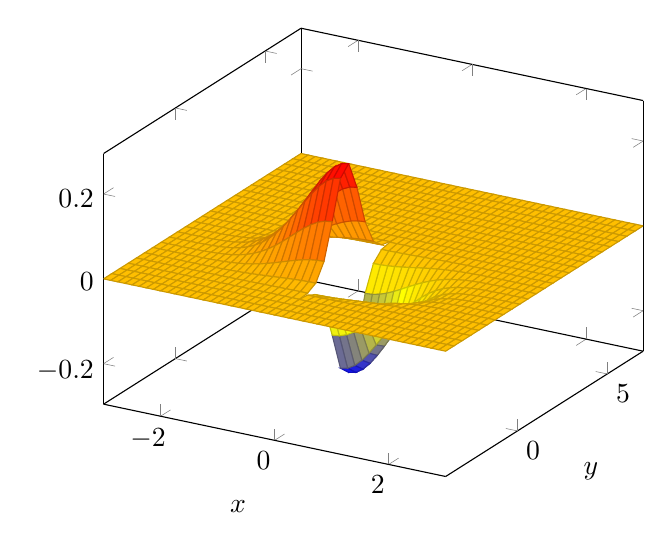
\begin{tikzpicture}
					\begin{axis}[
						view={30}{30},
						xlabel=$x$, ylabel=$y$
					]
					\addplot3[surf, domain =3:0, domain y=-4:7] {-1/4*exp(-x^2-y^2)};
					\addplot3[surf, domain =-3:0, domain y=-4:7] {1/4*exp(-x^2-y^2)};
					\end{axis}
				\end{tikzpicture}
			}
		\end{subfigure}
		\begin{subfigure}{.49\textwidth}
			\centering
			\resizebox{\linewidth}{!}{
				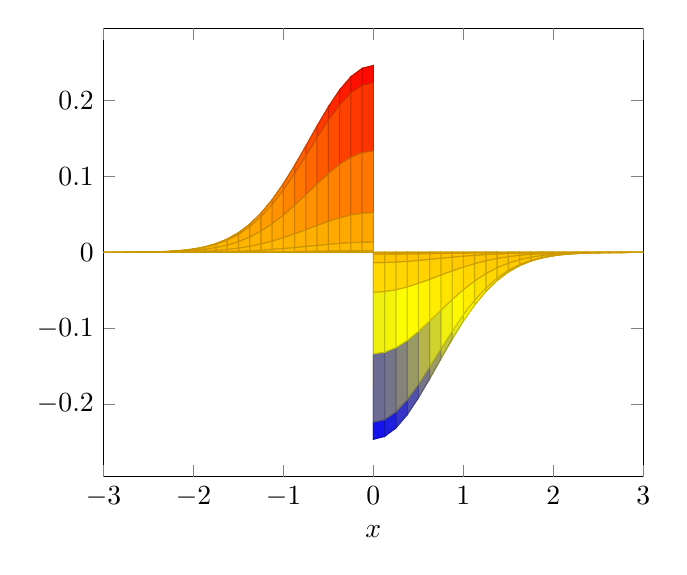
\begin{tikzpicture}
					\begin{axis}[
						view={0}{0},
						xlabel=$x$, ylabel=$y$
					]
					\addplot3[surf, domain =3:0, domain y=-4:7] {-1/4*exp(-x^2-y^2)};
					\addplot3[surf, domain =-3:0, domain y=-4:7] {1/4*exp(-x^2-y^2)};
					\end{axis}
				\end{tikzpicture}
			}
		\end{subfigure}
	\end{figure}
\end{example}
\begin{exercise}
	Sia $f:\R^2 \mapsto \R^m$ derivabile in $x_0$, con $x_0 \in \R^2$. Sia $g:\R^2 \mapsto \R^m$ definita da $g(x,y) = f(y,x)$\\
	Come sono legate le derivate parziali di $f$ e $g$ in $x_0$?
	% TODO solution
\end{exercise}
\begin{exercise}
	Sia $f:A \mapsto \R$ con $A \subseteq \R^n$, derivabile in $x_0 \in \circdot{A}$ . Determinare le derivate parziali in $x_0$ delle funzioni
	\begin{itemize}
		\item $F:A \mapsto \R^2$ definita da $\bigl( f(x), f(x) \bigr)$
		\item $G:A \times A \mapsto \R$ definita da $G(x,y) = f(x) + f(y)$
	\end{itemize}
	% TODO solution
\end{exercise}
\begin{proposition}
	Siano $A \subseteq \R^n$ e $x_0 \in \circdot{A}$. $f$ è \textbf{derivabile parzialmente} rispetto alla $i$-esima coordinata se e solo \textbf{se esiste} finito il limite
	\begin{equation}
		\label{eq:deriv_i_esima}
		\lim\limits_{t \to 0} \frac{f(x_1,\;\dotsc\;,x_i+t,\;\dotsc\;,x_n) - f(x_1,\;\dotsc\;,x_i,\;\dotsc\;,x_n)}{t}
	\end{equation}
	\begin{proof}
		Da \fullref{def:deriv_direz}, sceglendo $v = e_i$ della base canonica si ottiene la \cref{eq:deriv_i_esima}
	\end{proof}
\end{proposition}
\begin{exercise}
	\label{ex:funz_derivabili}
	Formulare in modo rigoroso e dimostrare:
	\begin{enumerate}
		\item La somma di funzioni parzialmente derivabili è parzialmente derivabile.
		\item La composizione di funzioni parzialmente derivabili è parzialmente derivabile.
		\item Prodotto e rapporto, quando definiti, di funzioni parzialmente derivabili sono funzioni parzialmente derivabili.
	\end{enumerate}
	% TODO solution
\end{exercise}
\begin{example}
	Sia $f: \R^2 \mapsto \R^3$ data da
	\begin{equation*}
		f(x,y) =
		\begin{bmatrix}
			2x + 3y\\
			\sin (xy^2)\\
			e^{xy}
		\end{bmatrix}
	\end{equation*}
	La funzione $f$ è derivabile parzialmente su tutto $\R^2$. Inoltre
	\[
		\frac{\partial f}{\partial x}(x,y) =
		\begin{bmatrix}
			2\\
			y^2 \cos (xy^2)\\
			y e^{xy}
		\end{bmatrix}
		\qquad\qquad
		\frac{\partial f}{\partial y}(x,y) =
		\begin{bmatrix}
			3\\
			2xy \cos (xy^2)\\
			x e^{xy}
		\end{bmatrix}
	\]
\end{example}

\begin{proposition}
	Siano $A \subseteq \R^n$, $x_0 \in \circdot{A}$ e $v \in \R^n$ con $v \neq 0$. Sia $f: A \mapsto \R^m$, allora
	\begin{equation*}
		\begin{gathered}
			f \text{ è \textbf{Derivabile} in $x_0$ nella direzione $v$}\\
			\iff\\
			\forall i = 1,\;\dotsc\;,m \quad \text{la \textbf{componente} $f_i$ \textbf{è derivabile} in $x_0$ nella direzione $v$}
		\end{gathered}
	\end{equation*}
	\begin{proof}
		Applicando \fullref{prop:succ_conv_se_comp_conv} e \fullref{prop:cont_e_cont_per_succ} % TODO proper proof. This does not make sense as of now, I know.
	\end{proof}
\end{proposition}
\begin{exercise}
	\label{ex:deriv_non_impl_cont}
	La derivabilità in ogni direzione non implica la continuità. Verificare che la funzione
	\[\funcdef{f}{\R^2}{\R}{(x,y)}
	{
		\begin{cases}
			1 \qquad \text{se } y = x^2 \text{ e } x \neq 0\\
			0 \qquad \text{altrimenti}
		\end{cases}
	}\]
	ammette nell'origine derivate direzionali in ogni direzione ma che \textit{non} è continua nell'origine.
	\begin{figure}[H]
		\begin{subfigure}{.49\textwidth}
			\centering
			\resizebox{\linewidth}{!}{
				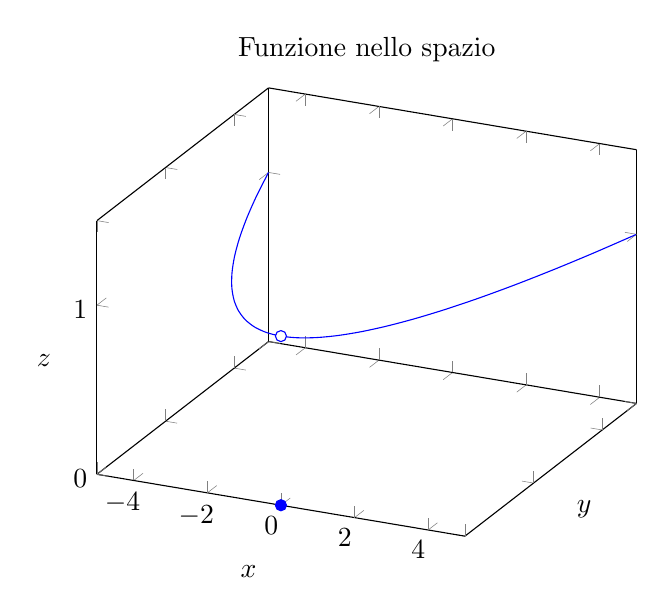
\begin{tikzpicture}
					\begin{axis}[
						title={Funzione nello spazio},
						xlabel=$x$, ylabel=$y$, zlabel=$z$, zlabel style={rotate=-90},
						yticklabels={,,},
						samples y=0,
						zmin = 0, zmax = 1.5
					]
					\addplot3 [smooth, color=blue] (x,x^2,1);
					\addplot3 [color=blue, fill=white, only marks,mark=*] coordinates{(0,0,1)};
					\addplot3 [color=blue, only marks, mark=*] coordinates{(0,0,0)};
					\end{axis}
				\end{tikzpicture}
			}
		\end{subfigure}
		\begin{subfigure}{.49\textwidth}
			\centering
			\resizebox{\linewidth}{!}{
				\begin{tikzpicture}
					\node at (3.4, .2) {$0$};

					\node at (2.1, 1.1) {$1$};
					\node at (4.8, 1.1) {$1$};
					\node at (1.2, 2.5) {$1$};
					\node at (5.65, 2.5) {$1$};
					\node at (.4, 4.5) {$1$};
					\node at (6.5, 4.5) {$1$};

					\node at (1.7, .2) {$0$};
					\node at (6, .6) {$0$};
					\node at (2.6, 2.2) {$0$};
					\node at (5, 3) {$0$};
					\node at (3.2, 4.3) {$0$};
					\node at (1.8, 5) {$0$};
					\begin{axis} [
						title={Valori della $z$},
						axis lines = center,
						xlabel=$x$, ylabel=$y$,
						xticklabels={,,}, yticklabels={,,},
						ymin = -1
					]
						\addplot[color=blue!70, smooth] {x^2};
					\end{axis}
				\end{tikzpicture}
			}
		\end{subfigure}
	\end{figure}

	\begin{solution}
		Le derivate direzionali sono
		\begin{align*}
			\partial_x f(0,0) &= \lim\limits_{t \to 0} \frac{f(0+t,0)-f(0,0)}{t} = 0\\
			\partial_y f(0,0) &= \lim\limits_{t \to 0} \frac{f(0,0+t)-f(0,0)}{t} = 0\\
			D_v f(0,0) &= \lim\limits_{t \to 0} \frac{f(0+t_1,0+t_2)-f(0,0)}{t} = 0
		\end{align*}
		Dunque, per ogni derivata parziale o direzionale in $(0,0)$ il valore della derivata sarà $0$.\\
		D'altro canto $f$ in $0$ \textit{non} è continua in $(0,0)$, quindi si è verificato che la derivabilità non implichi la continuità con $\dim A > 1$
	\end{solution}
\end{exercise}
\begin{exercise}
	Esibire una funzione $f: \R^2 \mapsto \R$ che ammetta in (almeno) un punto una derivata parziale rispetto ad $x$ ma non rispetto a $y$
	\begin{solution}
		La
		\[\funcdef{f}{\R^2}{\R}{(x,y)}{x+\sqrt{y}}\]
		È derivabile parzialmente rispetto a $x$ ma non rispetto a $y$ in $(0,0)$, infatti
		\begin{align*}
			\partial_x f(0,0) &= \lim\limits_{t \to 0} \frac{f(0+t,0)-f(0,0)}{t} = \frac{t-0}{t} = 1\\
			\partial_y f(0,0) &= \lim\limits_{t \to 0} \frac{f(0,0+t)-f(0,0)}{t} = \frac{\sqrt{t}-0}{t} = +\infty \implies \nexists \text{ limite finto}
		\end{align*}
	\end{solution}
\end{exercise}

\section{Derivata Totale}
\begin{theorem}[di Lagrange]\leavevmode\vspace*{-\baselineskip}
	\label{teo:lagrange}
	\begin{note}
		Questo teorema viene trattato approfonditamente nel corso di Analisi 1 e si applica solo a funzioni $\R^1 \mapsto \R^1$, qui verrà solo riportato rapidamente l'enunciato
	\end{note}
	\begin{note}
		Il \textbf{Teorema di Lagrange} è conosciuto anche come \textbf{Teorema del Valor Medio Differenziale}
	\end{note}
	Sia $f: \intervalclose{a}{b} \mapsto \R$ una funzione \textbf{Continua} nell'intervallo chiuso $\intervalclose{a}{b}$ e \textbf{Derivabile} nell'intervallo aperto $\intervalopen{a}{b}$. Allora esiste almeno un punto
	\[c \in \intervalopen{a}{b} : f'(c) = \frac{f(b)-f(a)}{b - a}\]
	O, alternativamente, nella forma
	\[\xi \in \intervalopen{0}{1} : f'(x_0 + \xi h) = \frac{f(x_0 + h)-f(x_0)}{h}\]
\end{theorem}
\begin{definition}[o piccolo]
	\label{def:o_piccolo}
	Siano $A \subseteq \R^n$ e $x_0 \in \circdot{A}$. Siano $f,g: A \mapsto \R^m$ due funzioni.
	\[f=o(g) \text{ per } x \to x_0 \qquad \bydef \qquad \lim\limits_{x \to x_0} \frac{\norm{f(x)}}{\norm{g(x)}}\]
	che si legge $f$ è \textbf{o piccolo} di $g$.
	\begin{note}
		Scrivere $f(x) = o(x^k)$ per $x \to 0$ significa che $f = o(g)$ con $g = x^k$
	\end{note}
	\begin{note}
		Con $o(1)$ per $x \to x_0$ si intende una qualunque funzione tendente a $0$ per $x \to x_0$.
	\end{note}
\end{definition}
\begin{exercise}
	Perché son state utilizzate le norme nella \fullref{def:o_piccolo}?
	\begin{solution}
		Perché l'operazione di divisione è sensata solo tra due scalari, non tra vettori.
	\end{solution}
\end{exercise}
\begin{exercise}
	Quali tra le seguenti uguaglianze sono vere? (In tutte, $x \to 0$)
	\begin{itemize}
		\begin{minipage}{0.33\linewidth}
			\item $o(x) = o(x) + o(x)$
			\item $o(x^2) = o(x) \cdot o(x)$
			\item $o(x^2) = o(x) - o(x)$
		\end{minipage}
		\begin{minipage}{0.33\linewidth}
			\item $\sqrt{x} = o(x)$
			\item $o(x) = \abs{o(x)}$
			\item $x = o(\sqrt{x})$
		\end{minipage}
		\begin{minipage}{0.33\linewidth}
			\item $o(x) = 10^6 o(x)$
			\item $x + x^2 = o(x)$
			\item $x = o(x + x^2)$
		\end{minipage}
	\end{itemize}
\end{exercise}
La seguente definizione è da ritenersi già nota da Analisi 1
\begin{definition}[Derivata in $\R$]
	Siano $A \subseteq \R$ e $x_0 \in \circdot{A}$. Sia $f: A \mapsto \R$
	\[f \text{ \textbf{Derivabile} in } x_0 \quad \bydef \quad \lim\limits_{h \to 0} \frac{f(x_0 + h) - f(x_0)}{h} \text{  esiste finito}\]
\end{definition}

Direttamente dalla nozione di Analisi 1 di derivata, si ottiene la seguente relazione tra derivata e coefficiente angolare della retta tangente in un punto
\begin{proposition}[Derivata Analisi 1]
	\label{prop:deriv_analisi_1}
	Siano $A \subseteq \R$ e $x_0 \in \circdot{A}$. Sia $f: A \mapsto \R$
	\begin{equation*}
		\begin{gathered}
			f \text{ è derivabile in } x_0\\
			\iff\\
			\exists m \in \R:\; f(x_0+h) = f(x_0) + mh +o(h) \text{ per } h \to 0
		\end{gathered}
	\end{equation*}
	\begin{proof}
		\begin{align*}
			& f \text{ è derivabile in } x_0\\
			\iff & \lim\limits_{h \to 0} \frac{f(x_0 + h) - f(x_0)}{h} \text{  esiste finito}\\
			\iff & \exists m \in \R:\; \lim\limits_{h \to 0} \frac{f(x_0 + h) - f(x_0)}{h} = m\\
			\iff & \exists m \in \R:\; \lim\limits_{h \to 0} \frac{f(x_0 + h) - f(x_0)}{h} - m = 0\\
			\iff & \exists m \in \R:\; \lim\limits_{h \to 0} \frac{f(x_0 + h) - f(x_0) -mh}{h} = 0
			\shortintertext{Per la nota alla \fullref{def:o_piccolo}}
			\iff & \exists m \in \R:\; f(x_0 + h) - f(x_0) -mh = o(h) \text{ per } h \to 0\\
			\iff & \exists m \in \R:\; f(x_0 + h) = f(x_0) -mh + o(h) \text{ per } h \to 0
		\end{align*}
	\end{proof}
\end{proposition}

\noindent Analogamente a quanto fatto nella \fullref{prop:deriv_analisi_1}, si definisce
\begin{definition}[Differenziale]
	\label{def:differenz}
	Siano $A \subseteq \R^n$ e $x_0 \in \circdot{A}$. Sia $f: A \mapsto \R^m$
	\begin{equation*}
		\begin{gathered}
			f \text{ è \textbf{Differenziabile} in } x_0\\
			\bydef\\
			\exists M \in \mat (m \times n):\; f(x_0 + h) = f(x_0) + Mh + o(h) \text{ per } h \to 0
		\end{gathered}
	\end{equation*}
	La matrice $M$ è la \textbf{Derivata Totale} di $f$ calcolata in $x_0$ e si indica con $Df(x_0)$. $Df(x_0)$ è l'applicazione \textit{lineare} che meglio approssima la variazione di $f$ nelle vicinanze di $x_0$.
	\begin{note}
		Verrà spiegato più avanti in \fullref{coro:se_diff_deriv_parz} un metodo pratico di calcolo della Derivata Totale.
	\end{note}
\end{definition}
\begin{observation}[Matrici Derivata Totale Particolari]
	\label{obs:matr_deriv_tot}
	Data la matrice $Df(x_0)$ con $m$ righe e $n$ colonne:
	\begin{itemize}
		\item Se $n = 1$ e $m = 1$ $Df(x_0)$ è \textbf{Derivata} di Analisi 1, uno scalare
		\item Se $n > 1$ e $m = 1$ $Df(x_0)$ è \textbf{Gradiente} di $f$ e si indica con $\nabla f(x_0)$ (\textit{nabla} $f$) o $\grad f(x_0)$
		\item Se $n = 1$ e $m > 1$ $Df(x_0)$ è \textbf{Vettore Tangente} alla $f$
		\item Se $n > 1$ e $m > 1$ $Df(x_0)$ è \textbf{Matrice Jacobiana} di $f$ e si può anche indicare con $J_f(x_0)$
	\end{itemize}
	Come si vedrà in \fullref{coro:se_diff_deriv_parz}, il Gradiente della \textit{i-esima} variabile è la \textit{i-esima} colonna di $Df(x_0)$.\\
	Il Vettore Tangente della \textit{j-esima} variabile è invece la \textit{j-esima} riga di $Df(x_0)$.
\end{observation}
\begin{example}
	Esempi relazioni tra Derivata Totale e derivate parziali
	\begin{align*}
		n = 2 \quad m = 1 \qquad & Df =
		\begin{bmatrix}
			\frac{\partial f}{\partial x} & \frac{\partial f}{\partial y}
		\end{bmatrix}\\
		n = 3 \quad m = 1 \qquad & Df =
		\begin{bmatrix}
			\frac{\partial f}{\partial x} & \frac{\partial f}{\partial y} &  \frac{\partial f}{\partial z}
		\end{bmatrix}\\
		n = 1 \quad m = 2 \qquad & Df =
		\begin{bmatrix}
			\frac{\partial f_1}{\partial x}\\[1ex]
			\frac{\partial f_2}{\partial x}
		\end{bmatrix}\\
		n = 2 \quad m = 2 \qquad & Df =
		\begin{bmatrix}
			\frac{\partial f_1}{\partial x} & \frac{\partial f_1}{\partial y}\\[1ex]
			\frac{\partial f_2}{\partial x} & \frac{\partial f_2}{\partial y}
		\end{bmatrix}\\
		n > 2 \quad m > 2 \qquad & Df =
		\begin{bmatrix}
			\frac{\partial f_1}{\partial x_1} & \frac{\partial f_1}{\partial x_2} & \dots & \frac{\partial f_1}{\partial x_n}\\[1ex]
			\frac{\partial f_2}{\partial x_1} & \frac{\partial f_2}{\partial x_2} & \dots & \frac{\partial f_2}{\partial x_n}\\[1ex]
			\vdots & \vdots & \ddots & \vdots\\[1ex]
			\frac{\partial f_m}{\partial x_1} & \frac{\partial f_m}{\partial x_2} & \dots & \frac{\partial f_m}{\partial x_n}
		\end{bmatrix}\\
	\end{align*}
\end{example}
\begin{exercise}
	Perché non è stata data una definizione di derivata attraverso il limite del rapporto incrementale?
	% TODO solution
\end{exercise}
\begin{example}
	Siano $M \in \mat(m \times n)$ una matrice fissata, $f: \R^n \mapsto \R^m$ data da $f(x) = Mx$.\\
	Allora $f$ è differenziabile ovunqe e per ogni $x_0 \in \R$ si ha $Df(x_0) = M$
\end{example}
\begin{proposition}[Unicità della Derivata Totale]
	\label{prop:unic_deriv_tot}
	Siano $A \subseteq \R^n$, $x_0 \in \circdot{A}$, $f: A \mapsto \R^m$ e $M_1, M_2 \in \mat(m \times n)$
	\begin{equation*}
		\left.
		\begin{array}{l}
			M_1 \text{ derivata totale di } f \text{ in } x_0\\
			M_2 \text{ derivata totale di } f \text{ in } x_0
		\end{array}
		\right\}
		\implies
		M_1 = M_2
	\end{equation*}
	\begin{proof}
		Sia $h \in \R$. Fissato un vettore $e_i$ della base canonica di $\R^n$
		\begin{align*}
			M_2 e_i - M_1 e_1 &=\\
			\shortintertext{Moltiplicando e dividendo per $h$}
			&= \frac{1}{h} M_2 e_i h - \frac{1}{h} M_1 e_i h\\
			&= \frac{1}{h} [M_2 e_i h - M_1 e_i h]
			\shortintertext{Grazie alla \fullref{def:differenz}}
			&= \frac{1}{h} [f(x_0 + h e_i) - f(x_0) + o(h)] - \frac{1}{h} [f(x_0 + h e_i) - f(x_0) + o(h)]\\
			&= o(h) \text{ per } t \to 0
		\end{align*}
		Passando al limite per $t \to 0$, si deduce che le applicazioni lineari $M_1$ e $M_2$ hanno le stesse immagini sui vettori della base canonica, quindi coincidono.
	\end{proof}
\end{proposition}
\begin{proposition}
	Siano $A \subseteq \R^n$, $x_0 \in \circdot{A}$ e $f:A \mapsto \R^m$
	\[f \text{ \textbf{Differenziabile} in } x_0 \implies f \text{ \textbf{Continua} in } x_0\]
	\begin{proof}
		Per ipotesi $x_0 \in \circdot{A}$, dunque $x_0$ è di accumulazione. A questo punto, grazie alla \fullref{prop:f_cont_se_isol_o_accum} basta verificare che $\lim\limits_{x \to x_0} f(x) = f(x_0)$.
		Dalla \fullref{def:differenz}
		\[f(x_0 + h) = f(x_0) + Mh + o(h) \text{ per } h \to 0\]
		Quindi, posto $h = x - x_0$ ed essendo $M = Df(x_0)$ per \fullref{def:differenz}
		\[\lim\limits_{x \to x_0} f(x) = \lim\limits_{x \to x_0} \bigl[f(x_0) + Df(x_0)(x-x_0) + o(x - x_0)\bigr] = f(x_0)\]
	\end{proof}
\end{proposition}
\begin{proposition}
	\label{prop:se_diff_deriv_dir}
	Siano $A \subseteq \R^n$, $x_0 \in \circdot{A}$ e $f:A \mapsto \R^m$
	\[
		f \text{ \textbf{Differenziabile} in } x_0
		\implies
		\begin{cases}
			\begin{array}{c}
				f \text{ ammette ogni \textbf{Derivata Direzionale} in } x_0\\
				e\\
				\forall v \in \R^n \setminus \brackets{0} D_v f(x_0) = Df(x_0)v
			\end{array}
		\end{cases}
	\]
	\begin{proof}
		Sia $v \in \R^n$ non nullo. Partendo dalla \fullref{def:deriv_direz}
		\begin{align*}
			&\lim\limits_{t \to 0} \frac{f(x_0 + tv) - f(x_0)}{t}
			\shortintertext{Sostituendo ora $f(x_0 + tv)$ con il secondo membro della \fullref{def:differenz}, dopo aver posto $h = tv$}
			= &\lim\limits_{t \to 0} \frac{\cancel{f(x_0)} + Df(x_0)(tv) + o(tv) - \cancel{f(x_0)}}{t}\\
			= &\lim\limits_{t \to 0} \frac{Df(x_0)(tv)}{t} + \lim\limits_{t \to 0} \frac{o(tv)}{t}\\
			= &Df(x_0)v
		\end{align*}
	\end{proof}
\end{proposition}
\begin{corollary}
	\label{coro:se_diff_deriv_parz}
	Siano $A \subseteq \R^n$, $x_0 \in \circdot{A}$ e $f:A \mapsto \R^m$
	\[
		f \text{ \textbf{Differenziabile} in } x_0
		\implies
		\begin{cases}
			\begin{array}{c}
				f \text{ ammette ogni \textbf{Derivata Parziale} in } x_0\\
				e\\
				\frac{\partial f}{\partial x_i}(x_0) = Df(x_0) \cdot e_i
			\end{array}
		\end{cases}
	\]
	Dove $Df(x_0) \cdot e_i$ non è altro che
	\[
		Df(x_0) \cdot e_i =
		\begin{bmatrix}
			x_{11} & x_{12} & \dots & x_{1n}\\
			x_{21} & x_{22} & \dots & x_{2n}\\
			\vdots & \ddots & & \vdots\\
			x_{n1} & x_{n2} & \dots & x_{nn}\\
		\end{bmatrix}
		\cdot
		\begin{bmatrix}
			(0 & \dots & 1 & \dots & 0)
		\end{bmatrix}
		=
		\begin{bmatrix}
			0 & \dots & x_{1i} & 0\\
			0 & \dots & x_{2i} & 0\\
			\vdots & \ddots & & \vdots\\
			0 & \dots & x_{ni} & 0\\
		\end{bmatrix}
	\]
	Cioè l'\textit{i-esima} colonna della $Df(x_0)$, come da \fullref{obs:matr_deriv_tot}
	\begin{note}
		Per quanto detto, il presente corollario offre il principale metodo di calcolo della \textbf{Derivata Totale}\\
		Inoltre è anche una dimostrazione alternativa della \fullref{prop:unic_deriv_tot}
	\end{note}
	\begin{proof}
		Direttamente dalla \fullref{prop:se_diff_deriv_dir} e dalla \fullref{def:deriv_direz} (sezione sulle derivate parziali)
	\end{proof}
\end{corollary}
\begin{observation}
	Sia \fullref{prop:se_diff_deriv_dir} che \fullref{coro:se_diff_deriv_parz} non possono essere invertiti, come verificato in \fullref{ex:deriv_non_impl_cont}.
\end{observation}
\begin{corollary}
	Siano $A \subseteq \R^n$, $x_0 \in \circdot{A}$ e $f:A \mapsto \R^m$
	\[f \text{ \textbf{Differenziabile} in } x_0 \implies f \text{ \textbf{Derivabile} in } x_0\]
	\begin{proof}
		Mediante il \fullref{coro:se_diff_deriv_parz} si vede immediatamente che rispetta la \fullref{def:deriv_direz}
	\end{proof}
\end{corollary}
\begin{corollary}
	\label{coro:f_diff_con_matr_comp}
	Siano $A \subseteq \R^n$, $x_0 \in \circdot{A}$ e $f:A \mapsto \R^m$. Sia $f$ derivabile parzialmente in $x_0$ e sia $M$ la $Df(x_0)$, matrice dei coefficienti $M_{ij} = \frac{\partial f_i}{\partial x_j}$
	\begin{equation*}
		\begin{gathered}
			f \text{ \textbf{Differenziabile} in } x_0\\
			\iff\\
			f(x_0 + h) - f(x_0) - Mh = o(h) \text{ per } h \to 0
		\end{gathered}
	\end{equation*}
	\begin{proof}
		Direttamente dalla \fullref{def:differenz}, per mezzo del \fullref{coro:se_diff_deriv_parz}.
	\end{proof}
\end{corollary}
\begin{exercise}
	Verificare che, nel caso $n = 2$ ed $m = 1$ il \fullref{coro:f_diff_con_matr_comp} si scrive
	\begin{equation*}
		\begin{gathered}
			f \text{ \textbf{Differenziabile} in } x_0\\
			\iff\\
			f(x_0 + h, y_o + k) - f(x_0, y_0) -
			\begin{bmatrix}
				\frac{\partial f}{\partial x}(x_0, y_0) & \frac{\partial f}{\partial y}(x_0, y_0)
			\end{bmatrix}
			\cdot
			\begin{bmatrix}
				h\\
				k
			\end{bmatrix}
			= o(\sqrt{h^2 + k^2}) \text{ per } h, k \to 0
		\end{gathered}
	\end{equation*}
	% TODO solution
\end{exercise}
\begin{exercise}
	Scrivere il \fullref{coro:f_diff_con_matr_comp} nel caso $n = 3$ ed $m = 1$
	% TODO solution
\end{exercise}

\begin{theorem}[del Differenziale Totale]
	\label{teo:diff_tot}
	Siano $A \subseteq \R^n$, $x_0 \in \circdot{A}$ e $f:A \mapsto \R^m$.
	\[
		\left.
		\text{
			\begin{tabular}{c}
				Per $i = 1,\;\dotsc\;,m$ e $j = 1,\;\dotsc\;,n$\\
				$\frac{\partial f_i}{\partial x_j}$ è \textbf{definita} in un \textbf{intorno} di $x_0$ e \textbf{Continua} in $x_0$
			\end{tabular}
		}
		\right\}
		\implies\\
		f \text{ è \textbf{Differenziabile} in } x_0
	\]
	\vspace*{-\baselineskip}
	\begin{note}
		È specificata la necessità di continuità in un intorno di $x_0$ in quanto, come detto in \fullref{def:deriv_direz}, l'esistenza di derivate parziali non garantisce la continuità.
	\end{note}
	\begin{proof}
		Si può supporre $n = 2$ e $m = 1$ in quanto il caso più generale è del tutto analogo.\\
		È necessario verificare la \fullref{def:differenz}, dunque in $\R^n = \R^2$ si ha
		\begin{equation}
			\label{eq:deriv_tot_def_diff}
			f(x_0 + h, y_0 + k) = f(x_0, y_0) + Df(x_0, y_0) \begin{bmatrix}h\\k\end{bmatrix} + o(h,k) \text{ per } h,k \to 0
		\end{equation}
		Considerando solo i primi due addendi, aggiungendo e sottraendo la stessa quantità, si ottiene
		\begin{equation}
			\label{eq:teo_diff_tot_sommo_sottraggo}
			f(x_0 + h, y_0 + k) - f(x_0, y_0) = \underbrace{f(x_0 + h, y_0 + k) - f(x_0+h,y_0)}_{\text{(1)}} + \underbrace{f(x_0+h,y_0) - f(x_0, y_0)}_{\text{(2)}}
		\end{equation}
		Considerando la (1) e la (2) di \cref{eq:teo_diff_tot_sommo_sottraggo} come funzioni in una sola variabile, si può applicare il \fullref{teo:lagrange}
		\begin{itemize}
			\item La (1) rispetto a $y$, con $x_0 + h$ fissato
			\item La (2) rispetto a $x$, con $y_0$ fissato
		\end{itemize}
		Spostandosi lungo le direzioni parallele agli assi è possibile andare da $(x_0 + h, y_0 + k)$ a $(x_0, y_0)$
		\begin{center}
			\begin{tikzpicture}
				\pgfmathsetmacro\MAX{8}
				\pgfmathsetmacro\XZ{\MAX / 3 }
				\pgfmathsetmacro\YZ{\MAX / 3 }
				\pgfmathsetmacro\XZh{\MAX / 3 *2}
				\pgfmathsetmacro\YZk{\MAX / 3 *2}
				\coordinate (X0Y0) at (\XZ,\YZ);
				\coordinate (X0hY0) at (\XZh,\YZ);
				\coordinate (X0Y0k) at (\XZ,\YZk);
				\coordinate (X0hY0k) at (\XZh,\YZk);

				\draw[->] (0,0) -- (\MAX,0) node[anchor=north west] {$x$};
				\draw[->] (0,0) -- (0,\MAX) node[anchor=south east] {$y$};
				\draw[dotted] (\XZ,0) -- (\XZ,\MAX);
				\draw[dotted] (0,\YZ) -- (\MAX,\YZ);
				\draw[dotted] (\XZh,0) -- (\XZh,\MAX);
				\draw[dotted] (0,\YZk) -- (\MAX,\YZk);
				\draw node[anchor=north] at (\XZ,0) {$x_0$};
				\draw node[anchor=north] at (\XZh,0) {$x_0+h$};
				\draw node[anchor=east] at (0,\YZ) {$y_0$};
				\draw node[anchor=east] at (0,\YZk) {$y_0+k$};
				\draw node at (X0Y0) {$\bullet$};
				\draw node at (X0Y0k) {$\bullet$};
				\draw node at (X0hY0) {$\bullet$};
				\draw node at (X0hY0k) {$\bullet$};
				\draw node[anchor=north east] at (X0Y0) {$(x_0,y_0)$};
				\draw node[anchor=south east] at (X0Y0k) {$(x_0,y_0+k)$};
				\draw node[anchor=north west] at (X0hY0) {$(x_0+h,y_0)$};
				\draw node[anchor=south west] at (X0hY0k) {$(x_0+h,y_0+k)$};

				\draw[<-] (\XZ,\MAX*4/10) -- (\XZ,\MAX*6/10);
				\draw[<-] (\XZh,\MAX*4/10) -- (\XZh,\MAX*6/10);
				\draw[<-] (\MAX*4/10,\YZ) -- (\MAX*6/10,\YZ);
				\draw[<-] (\MAX*4/10,\YZk) -- (\MAX*6/10,\YZk);
			\end{tikzpicture}
		\end{center}
		Quindi, applicando il \fullref{teo:lagrange}:
		\[
			\exists \alpha, \beta \in \intervalopen{0}{1} \textbf{ per cui} \qquad
			\begin{array}{rrcl}
				\text{(1)} & f(x_0 + h, y_0 + k) - f(x_0 + h, y_0) &=& \frac{\partial f}{\partial y} (x_0 + h, y_0 + \beta k) k\\[1ex]
				\text{(2)} & f(x_0 + h, y_0) - f(x_0, y_0) &=& \frac{\partial f}{\partial x} (x_0 + \alpha h, y_0) h
			\end{array}
		\]
		Tornando alla \cref{eq:deriv_tot_def_diff}, si ottiene
		\begin{align*}
			&f(x_0 + h, y_0 + k) - f(x_0, y_0) - Df(x_0, y_0) \begin{bmatrix}h\\k\end{bmatrix}\\
			= &\underbrace{f(x_0 + h, y_0 + k) - f(x_0+h,y_0)}_{\text{(1)}} + \underbrace{f(x_0+h,y_0) - f(x_0, y_0)}_{\text{(2)}} - Df(x_0, y_0) \begin{bmatrix}h\\k\end{bmatrix}\\
			= &\underbrace{\frac{\partial f}{\partial y} (x_0 + h, y_0 + \beta k) k}_{\text{(1)}} + \underbrace{\frac{\partial f}{\partial x} (x_0 + \alpha h, y_0) h}_{\text{(2)}} - Df(x_0, y_0) \begin{bmatrix}h\\k\end{bmatrix}
			\shortintertext{Si esegue il prodotto tra matrice Derivata Totale e vettore, infine si separano i termini}
			= &	\left( \frac{\partial f}{\partial y} (x_0 + h, y_0 + \beta k) - \frac{\partial f}{\partial y} (x_0 + h, y_0) \right) k +
				\left( \frac{\partial f}{\partial x} (x_0 + \alpha h, y_0) - \frac{\partial f}{\partial x} (x_0, y_0)\right) h
		\end{align*}
		Si passa dunque alla norma
		\begin{align*}
			&\norm{f(x_0 + h, y_0 + k) - f(x_0, y_0) - Df(x_0, y_0) \begin{bmatrix}h\\k\end{bmatrix}}\\
			\shortintertext{Separando come fatto prima ed applicando la disguguaglianza triangolare}
			\leq &	\norm{\left( \frac{\partial f}{\partial y} (x_0 + h, y_0 + \beta k) - \frac{\partial f}{\partial y} (x_0 + h, y_0) \right) k} +
					\norm{\left( \frac{\partial f}{\partial x} (x_0 + \alpha h, y_0) - \frac{\partial f}{\partial x} (x_0, y_0)\right) h}
			\shortintertext{Per proprietà 4 da \fullref{def:norma}}
			= & \norm{\frac{\partial f}{\partial y} (x_0 + h, y_0 + \beta k) - \frac{\partial f}{\partial y} (x_0 + h, y_0)} \abs{k} +
				\norm{\frac{\partial f}{\partial x} (x_0 + \alpha h, y_0) - \frac{\partial f}{\partial x} (x_0, y_0)} \abs{h}
			\shortintertext{Presa ora la norma del vettore $(h,k)$, cioè $\norm{(h,k)} = \sqrt{h^2 + k^2}$, sicuramente $\abs{h} \leq \norm{(h,k)}$ e $\abs{k} \leq \norm{(h,k)}$, dunque}
			\leq &	\norm{\frac{\partial f}{\partial y} (x_0 + h, y_0 + \beta k) - \frac{\partial f}{\partial y} (x_0 + h, y_0)} \sqrt{h^2 + k^2} +
					\norm{\frac{\partial f}{\partial x} (x_0 + \alpha h, y_0) - \frac{\partial f}{\partial x} (x_0, y_0)} \sqrt{h^2 + k^2}
			\shortintertext{Essendo $h,k \to 0$ da \cref{eq:deriv_tot_def_diff} e graze alla continuità delle derivate, le due norme tendono a $0$. Inoltre, per \fullref{def:o_piccolo}}
			=\; &o(1) \sqrt{h^2 + k^2} \text{ per } \begin{bmatrix}h\\k\end{bmatrix} \to 0\\
			=\; &o(\sqrt{h^2 + k^2}) \text{ per } \begin{bmatrix}h\\k\end{bmatrix} \to 0
		\end{align*}
		Da cui la tesi, avendo verificato la \fullref{def:differenz}.
	\end{proof}
\end{theorem}
\begin{exercise}
	Data la funzione
	\[
		\funcdef{f}{\R}{\R}{x}{
			\begin{cases}
				\begin{array}{ll}
					x^2 \sin \frac{1}{x} & x \neq 0\\
					0 & x = 0
				\end{array}
			\end{cases}
		}
	\]
	Verificare che $f$ è differenziabile su $\R$ ma non ha derivata continua su $\R$.
	% TODO solution
\end{exercise}

\begin{definition}[Funzioni di Classe $\cntclass{1}$]
	Sia $A \subseteq \R^n$ un \textbf{Aperto}.
	\begin{center}
		$\cntclass{1}(A; \R^m)$ è l'insieme delle funzioni $f:A \mapsto \R^m$\\
		con \textbf{tutte} le \textbf{Derivate Parziali prime continue} in ogni punto di $A$
	\end{center}
	Si può anche leggere \textit{$f$ è di classe $\cntclass{1}$ su $A$ con valori in $\R^m$}.
\end{definition}
\begin{corollary}
	Sia $A \subseteq \R^n$ un \textbf{Aperto}. Se $f \in \cntclass{1}(A;\R^m)$ allora $f$ è \textbf{Differenziabile} su $A$.
	\begin{proof}
		Applicare la \fullref{teo:diff_tot}
	\end{proof}
\end{corollary}
\begin{proposition}
	\label{prop:cnt_class_components}
	Siano $m \in \N, m \geq 1$ e $A \subseteq \R^n$ un \textbf{Aperto}
	\[f \in \cntclass{1}(A; \R^m) \iff \forall i = 1,\;\dotsc\;, m \quad f_i \in \cntclass{1}(A;\R)\]
	\begin{proof}
		Immediata.
	\end{proof}
\end{proposition}
\begin{exercise}
	Dimostrare la \fullref{prop:cnt_class_components}.
	% TODO solution
\end{exercise}
\begin{exercise}
	Dimostrare che $\cntclass{1}(A;\R)$ non coincide con l'insieme delle funzioni differenziabili su $A$ con valori in $\R$.
	% TODO solution
\end{exercise}
\begin{proposition}
	\label{prop:if_df_lim_then_unif_cont}
	Siano $I \in \R$ un intervallo reale e $f(x)$ una funzione \textbf{Derivabile} in $I$. Se la $f'(x)$ è una \textbf{Funzione Limitata} in $I$, allora f è \textbf{Uniformemente Continua} in $I$ % Taken from http://www.batmath.it/matematica/an_uno/cont_unif/cont_unif.htm
	\begin{proof}
		Omessa. % TODO proof
	\end{proof}
\end{proposition}

\subsection{Regole di Derivazione}\label{sect:regole_deriv}
%TODO This section is a placeholder, the following proposition have to be rewritten
\proposition
\label{prop:diff_somma_diff}
Siano $f,g: A\subseteq \R^n \rightarrow \R^m$ e $x_0\in\circdot{A}$\\
$f$ differenziabile in $x_0$, $g$ differenziabile in $x_0$ allora $f+g$ differenziabile in $x_0$ e $D(f+g)(x_0) = Df(x_0)+Dg(x_0)$
\begin{proof}
	$f$ è differenziabile, allora $f(x_0+h)=f(x_0)+Df(x_0)h+o(h)$ per $h\rightarrow 0$\\
	anche $g$ lo è, quindi $g(x_0+h)=g(x_0)+Dg(x_0)h+o(h)$ per $h\rightarrow 0$\\
	sommando membro a membro si ottiene  $(f+g)(x_0+h)=(f+g)(x_0)+[Df(x_0)+Dg(x_0)]h+o(h)$ per $h\rightarrow 0$\\
	Questa è la definizione di differenziabilità, allora $f+g$ è differenziabile e $D(f+g)(x_0) = Df(x_0)+Dg(x_0)$
\end{proof}

\proposition
Sia $f: A\subseteq \R^n \rightarrow \R^m$ e $x_0\in\circdot{A}$ e $\lambda\in \R$\\
$f$ differenziabile in $x_0$ allora $\lambda f$ differenziabile in $x_0$ e $D(\lambda f)(x_0) = \lambda Df(x_0)$
\begin{proof}
	$f$ è differenziabile, allora $f(x_0+h)=f(x_0)+Df(x_0)h+o(h)$ per $h\rightarrow 0$\\
	valuto ora $(\lambda f)(x_0+h)=(\lambda f)(x_0)+\lambda Df(x_0)h+o(h)$ per $h\rightarrow 0$\\
	Questa è la definizione di differenziabilità, allora $\lambda f$ è differenziabile e $D(\lambda f)(x_0) = \lambda Df(x_0)$
\end{proof}

\proposition
Sia $g: A\subseteq \R^n \rightarrow \R^m$ e $x_0\in\circdot{A}$\\
Sia $f: B\subseteq \R^m \rightarrow \R^p$ e $g(x_0)\in\circdot{B}$\\
$f$ differenziabile in $g(x_0)$, $g$ differenziabile in $x_0$ allora $f\circ g$ differenziabile in $x_0$ e $D(f\circ g)(x_0) = Df(g(x_0))*Dg(x_0)$
\begin{proof}
	$g$ è differenziabile in $x_0$, allora $g(x_0+h)=f(x_0)+Dg(x_0)h+o(h)$ per $h\rightarrow 0$\\
	$f$ è differenziabile in $g(x_0)$ allora $g(g(x_0)+k)=f(g(x_0))+Df(g(x_0))k+o(k)$ per $k\rightarrow 0$\\
	valuto ora 
	\[(f\circ g)(x_0+h) = f(g(x_0+h)+Dg(x_0)h+o(h)) = \] 
	\[=f(g(x_0))+Df(g(x_0))(Dg(x_0)h+o(h))+o(Dg(x_0)h+o(h)) = \]
	\[=(f\circ g)(x_0) + Df(g(x_0))Dg(x_0)h+Df(g(x_0))o(h)+Dg(x_0)o(h)+o(h)\]
	
	con $h$ un vettore $n\times 1$\\
	con $Dg$ una matrice $m\times n$\\
	con $Df$ una matrice $p\times m$\\
	
	da rivedere un pochino ....
	
	Questa è la definizione di differenziabilità, allora $f\circ g$ è differenziabile e $D(f\circ g)(x_0) = Df(g(x_0))Dg(x_0)$
\end{proof}
\proposition DERIVATA DEL PRODOTTO

\subsection{La Formula degli Accrescimenti Finiti}
\begin{definition}[Segmento]
	\label{def:segmento}
	Siano $x_0,x_1 \in \R^n$, si dice \textbf{Segmento} di estremi $x_0$ e $x_1$ l'insieme che li unisce, cioè
	\[S = \brackets{tx_1+(1-t)x_0 \in \R^n:\; t \in \intervalclose{0}{1}}\]
\end{definition}
\begin{observation}
	La \fullref{def:segmento} può essere formulata in ogni spazio affine o vettoriale
\end{observation}
\begin{exercise}
	Dimostrare che ogni \textbf{Segmento} in $\R^n$ è \textbf{Compatto} e \textbf{Connesso}.
	\begin{solution}
		Posta
		\[\funcdef{\varphi}{\intervalclose{0}{1}}{\R^n}{t}{t x_1 + (1-t) x_0}\]
		\begin{itemize}
			\item $\intervalclose{0}{1} \subset \R^n$, essendo sottoinsieme di $\R^n$ chiuso e limitato, grazie alla \fullref{prop:compat_chius_lim_Rn}, è compatto. Inoltre, grazie al \fullref{teo:weier_generale}, $\varphi(\intervalclose{0}{1})$ è sicuramente compatto a sua volta, dunque il segmento $S$ è compatto.
			\item Dalla \fullref{prop:f_di_conn_cont_e_conn}, essendo $\varphi$ continua, il segmento $S$ è sicuramente Connesso.
		\end{itemize}
	\end{solution}
\end{exercise}
\begin{exercise}
	Ispirandosi alla \fullref{def:segmento} è possibile dare una possibile definizione di Semiretta uscente da $x_0$ e passante per $x_1$?
	\begin{solution}
		\[s = \brackets{x_0+(x_1-x_0)t \in \R^n: t \in \intervalclop{0}{+\infty} \;}\]
	\end{solution}
\end{exercise}
\begin{theorem}[degli Accrescimenti Finiti]
	\label{teo:accresc_fin}
	Sia $f \in \cntclass{1}(A;\R^m)$, con $A \subseteq \R^n$. Siano $x_0, x_1 \in \circdot{A}$ tali che il \textbf{Segmento} $S$ di estremi $x_0$ e $x_1$ sia \textbf{interamente contenuto} in $\circdot{A}$. Allora
	\begin{equation}
		\label{eq:accresc_fin}
		\norm{f(x_1) - f(x_0)} \leq \sup\limits_{\xi \in S} \norm{Df(\xi)} \cdot \norm{x_1-x_0}
	\end{equation}
	\begin{note}
		Con $\R^m = \R^1$ e $A \subseteq \R^1$ è come dire
		\[
			\abs{f(x_1) - f(x_0)} \leq M \cdot \abs{x_1 - x_0} \quad \text{con} \quad M = \sup \brackets{\text{\itshape\begin{tabular}{c}coefficiente angolare di tutte le\\rette tangenti alla curva\end{tabular}}}
		\]
		\begin{center}
			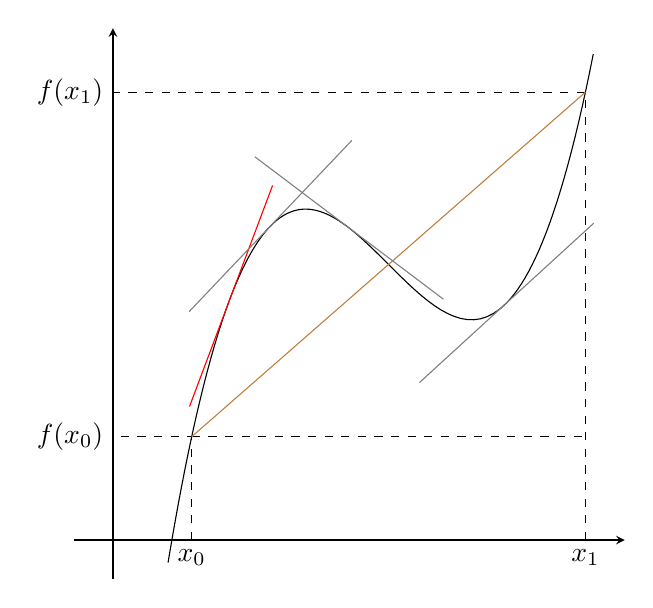
\begin{tikzpicture}[declare function = {curve(\x)=0.3*(\x-3.5)^3-\x+7; x_0=1; x_1=6;}]
				% Axes
				\draw[-stealth] (-0.5,0) -- (6.5,0);
				\draw[-stealth] (0,-0.5) -- (0,6.5);
				% Curve
				\draw[domain=.7:1.5] plot (\x,{curve(\x)}) {[turn] (-1.5,0) coordinate(t0) (1.5,0) coordinate(t1)}; % This is the most steep tangent
				\draw[domain=1.5:2] plot (\x,{curve(\x)}) {[turn] (-1.5,0) coordinate(t2) (1.5,0) coordinate(t3)};
				\draw[domain=2:3] plot (\x,{curve(\x)}) {[turn] (-1.5,0) coordinate(t4) (1.5,0) coordinate(t5)};
				\draw[domain=3:5] plot (\x,{curve(\x)}) {[turn] (-1.5,0) coordinate(t6) (1.5,0) coordinate(t7)};
				\draw[domain=5:6.1] plot (\x,{curve(\x)});
				% Dashed lines
				\foreach \x in {x_0,x_1}
				{\draw[dashed] (\x,0) node[below]{$\x$} |- (0,{curve(\x)}) node[left] {$f(\x)$};}
				\draw[dashed] (x_0,{curve(x_0)}) -- (x_1,{curve(x_0)});
				% Delta-y
				\draw[brown] ({x_0},{curve(x_0)}) -- ({x_1},{curve(x_1)});
				% Tangents
				\draw[red] (t0)--(t1);
				\draw[black!50] (t2)--(t3);
				\draw[black!50] (t4)--(t5);
				\draw[black!50] (t6)--(t7);
			\end{tikzpicture}
		\end{center}
	\end{note}
	\begin{proof}
		Si può dare per scontato che $x_1 \neq x_0$, in quanto, se $x_1 = x_0$ , allora $f(x_1) = f(x_0)$ e la \cref{eq:accresc_fin} diventerebbe $0 \leq 0$. La tesi sarebbe quindi verificata direttamente.\\
		Fissato un qualsiasi $v \in \R^m$, si definisce così la funzione $F$ legata ad $f$ tramite la \fullref{def:segmento}:
		\begin{equation}
			\label{eq:accresc_fin_F}
			\funcdef{F}{\intervalclose{0}{1}}{\R}{t}{v \cdot f \bigl( t x_1 + (1-t)x_0 \bigr)}
		\end{equation}
		\begin{note}
			Nella \cref{eq:accresc_fin_F},  $\cdot$  è Prodotto Scalare tra due vettori di dimensione $\R^m$, dunque il risultato è correttamente uno scalare.
		\end{note}
		$F$ è continua e derivabile sull'intervallo di definizione $\intervalclose{0}{1}$. È dunque possibile utilizzare il \fullref{teo:lagrange}, che garantisce:
		\[\exists c \in \intervalopen{0}{1}: \quad F(1) - F(0) = F'(c) \; (1-0)\]
		Tornando dunque a $f$ dalla definizione di $F$
		\[v \cdot f(x_1) - v \cdot f(x_0) = v \cdot Df\bigl( cx_1 + (1-c)x_0 \bigr) (x_1 - x_0)\]
		Ricordando che la $F$ è a valori in $\R$, si può calcolare il valore assoluto mantenendo l'uguaglianza
		\[\abs{v \cdot f(x_1) - v \cdot f(x_0)} = \abs{v \cdot Df\bigl( cx_1 + (1-c)x_0 \bigr) (x_1 - x_0)}\]
		Essendo il secondo membro il valore assoluto di un prodotto scalare, si può applicare ad esso la \textbf{Disuguaglianza di Cauchy-Schwarz} ed ottenere
		\[\abs{v \cdot \bigl( f(x_1) - f(x_0) \bigr)} \leq \norm{v} \cdot \norm{Df\bigl( cx_1 + (1-c)x_0 \bigr) (x_1 - x_0)}\]
		Dunque, seaparando ulteriorimente le norme si arriva alla:
		\begin{equation}
			\label{eq:accr_fin_norm}
			\abs{v \cdot \bigl( f(x_1) - f(x_0) \bigr)} \leq \norm{v} \cdot \norm{Df\bigl( cx_1 + (1-c)x_0 \bigr)} \cdot \norm{x_1 - x_0}
		\end{equation}

		Essendo, come detto all'inzio, $f(x_1) \neq f(x_0)$ è ora possibile scegliere un $v$ "comodo", come:
		\[v = \frac{1}{\norm{f(x_1) - f(x_0)}} \cdot \bigl( f(x_1) - f(x_0) \bigr)\]
		\begin{note}
			La norma di $v$, grazie poi alla proprietà 4 da \fullref{def:norma}, è
			\begin{align*}
				\norm{v} &= \norm{
					\underbrace{\frac{1}{\norm{f(x_1) - f(x_0)}}}_{\text{Scalare}}
					\cdot
					\underbrace{\bigl( f(x_1) - f(x_0) \bigr)}_{\text{Vettore}}
					}\\
				&= \abs{\frac{1}{\norm{f(x_1) - f(x_0)}}} \cdot \norm{\bigl( f(x_1) - f(x_0) \bigr)}\\
				&= \frac{1}{\norm{f(x_1) - f(x_0)}} \cdot \norm{\bigl( f(x_1) - f(x_0) \bigr)}\\
				&= 1
			\end{align*}
		\end{note}
		Sostituendo dunque in \cref{eq:accr_fin_norm} si ottiene
		\[\norm{\frac{1}{\norm{f(x_1) - f(x_0)}} \cdot \bigl( f(x_1) - f(x_0) \bigr) \cdot \bigl( f(x_1) - f(x_0) \bigr)} \leq \cdot \norm{Df\bigl( cx_1 + (1-c)x_0 \bigr)} \cdot \norm{x_1 - x_0}\]
		Dal punto 3 di \fullref{ex:sp_norm}, si ottiene
		\[\norm{\frac{1}{\norm{f(x_1) - f(x_0)}} \cdot \norm{f(x_1) - f(x_0)}^2} \leq \norm{Df\bigl( cx_1 + (1-c)x_0 \bigr)} \cdot \norm{x_1 - x_0}\]
		Da cui
		\[\norm{f(x_1) - f(x_0)} \leq \norm{Df\bigl( cx_1 + (1-c)x_0 \bigr)} \cdot \norm{x_1 - x_0}\]
		e passando al $\sup$ su $t \in \intervalopen{0}{1}$ si ottiene la tesi.
	\end{proof}
\end{theorem}
Il seguente esercizio mostra come il \fullref{teo:lagrange} non possa essere esteso al caso di funzioni a valori in $\R^n$ con $n > 1$.
\begin{exercise}
	Sia $f: \R \mapsto \R^2$ data da $f(t) = (\cos t, \sin t)$. Mostrare che non esiste nessun numero reale $c$ tale che
	\[f(2 \pi) - f(0) = Df(c) \cdot 2 \pi\]
\end{exercise}

\begin{definition}[Insieme Convesso]
	\label{def:convesso}
	Sia $C \subseteq \R^n$
	\begin{equation*}
		\begin{gathered}
			C \text{ è \textbf{Convesso}}\\
			\bydef\\
			\forall x_0,y_1 \in C \quad \brackets{tx_1+(1-t)x_0:\; t \in \intervalclose{0}{1}} \subseteq C
		\end{gathered}
	\end{equation*}
	Cioè un insieme è Convesso se, dati qualsiasi due suoi punti, contiene anche il segmento che li congiunge.
\end{definition}
\begin{exercise}
	Dimostrare la \fullref{prop:convesso_deriv_par_lim_allora_lips}
	% TODO solution
\end{exercise}
\begin{exercise}
	In $\R^n$ dimostrare che ogni segmento è convesso, così come anche ogni sfera.\\
	Esibire un esempio di insieme non convesso.
	% TODO solution
\end{exercise}
\begin{corollary}
	\label{coro:convess_nabla_0_f_const}
	Siano $A \subseteq \R^n$ e $f: A \mapsto \R$
	\[
		\left.
			\begin{array}{l}
				A \text{ \textbf{Aperto Convesso}}\\
				f \text{ \textbf{Differenziabile} in } A\\
				\forall x \in A \quad \nabla f(x) = 0
			\end{array}
		\right\}
		\implies\\
		f \text{ è \textbf{Costante} su } A
	\]
	\vspace*{-\baselineskip}
	\begin{note}
		Come da \fullref{obs:matr_deriv_tot}, $\nabla f(x) = Df(x) \in \mat (1 \times n)$, cioè un vettore riga.
	\end{note}
	\begin{proof}
		Se $\nabla f(x) = Df(x) = 0$, la \cref{eq:accresc_fin} da \fullref{teo:accresc_fin} diventa
		\begin{equation*}
			\begin{gathered}
				\norm{f(x_1) - f(x_0)} \leq \sup\limits_{\xi \in S} 0 \cdot \norm{x_1-x_0}\\
				\norm{f(x_1) - f(x_0)} \leq 0\\
				f(x_1) = f(x_0)
			\end{gathered}
		\end{equation*}
	\end{proof}
\end{corollary}
\begin{exercise}
	Dimostrare che un insieme \textbf{Convesso} è anche \textbf{Connesso}.\\
	Esibire un controesempio al viceversa.
	\begin{solution}
		Supponendo, per assurdo, $C \in \R^n$ sconnesso. In questo caso, per \fullref{def:connesso}, esistono due insiemi separati $S_1$ e $S_2$ che costituiscono $C$, inoltre $S_1 \cup S_2 = C$ e $S_1 \cap S_2 = \emptyset$. Questo implica che
		\[\exists t \in \intervalclose{0}{1}:\; \forall x_1 \in S_1 \text{ e } \forall x_2 \in S_2 \quad tx_1 + (1-t)x_2 \notin S_1 \text{ e contemporaneamente } \notin S_2\]
		Questo implica la non convessità di $C$ - \textit{Assurdo}.\\

		Preso il cerchio di raggio unitario $S = {(x,y): x^2 + y^2 = 1}$, questo verifica la \fullref{def:connesso} ma sicuramente non la \fullref{def:convesso}.
	\end{solution}
\end{exercise}
\begin{exercise}
	Esibire esempi di insiemi convessi/non convessi e aperti/chiusi, limitati/illimitati.
	% TODO solution
\end{exercise}

\begin{definition}[Funzione Convessa]
	Sia $I$ un intervallo reale e $f:\; I \mapsto \R$.
	\begin{equation*}
		f \text{ è \textbf{Convessa}}
		\quad \bydef \quad
		\begin{cases}
			\forall x_0, x_1 \in I,\; \forall t \in \intervalclose{0}{1}\\
			f \bigl( (1-t)x_0 + t x_1 \bigr) \leq (1-t) f(x_0) + t f(x_1)
		\end{cases}
	\end{equation*}
	Cioè se il segmento che congiunge due qualsiasi punti del suo grafico si trova al di sopra del grafico stesso.
\end{definition}
\begin{exercise}
	Verificare che $f$ è \textbf{Convessa} se e solo se il suo \textbf{Epigrafo} (cioè l'insieme di punti che stanno al di sopra o sul grafico della funzione)
	è un sottoinsieme \textbf{Convesso} di $\R^2$ nel senso della \fullref{def:convesso}.
	% TODO solution
\end{exercise}
\begin{proposition}
	Siano $A \subseteq \R^n$ e $f: A \mapsto \R$
	\[
		\left.
			\begin{array}{l}
				A \text{ \textbf{Aperto Connesso}}\\
				f \text{ \textbf{Differenziabile} in } A\\
				\forall x \in A \quad \nabla f(x) = 0
			\end{array}
		\right\}
		\implies\\
		f \text{ è \textbf{Costante} su } A
	\]
	\vspace*{-\baselineskip}
	\begin{note}
		Si sta parlando di insiemi Co\textbf{nn}essi
	\end{note}
	\begin{proof}
		Sia $x_0 \in A$. Per la \fullref{prop:polig_in_aperto_connesso}, ogni punto $x \in A$ può essere unito a $x_0$ con una poligonale interamente contenuta in $A$ dai lati paralleli agli assi. A questo punto è possibile applicare il \fullref{teo:accresc_fin} ad ogni segmento della poligonale ed, essendo $\nabla f(x) = 0$, come in \fullref{coro:convess_nabla_0_f_const}, la $f$ è costante.
	\end{proof}
\end{proposition}

\section{Derivate Seconde}
Quanto detto circa le derivate prime può essere ripetuto introducendo derivate di ordine superiore.
\begin{definition}[Derivate Parziali Seconde]
	Sia $f: A \mapsto \R^m$ con $A \subseteq \R^n$ derivabile parzialmente in $x_0$ lungo $e_i$.\\
	Se la funzione $\frac{\partial f}{\partial x_i}$ è a sua volta derivabile parzialmente in $x_0$, questa volta lungo $e_j$, allora la quantità
	\[
		\frac{\partial}{\partial x_j} \frac{\partial f}{\partial x_i} (x_0)
		\quad \bydef \quad
		\begin{array}{c}
			\text{ è la \textbf{Derivata Parziale Seconda}}\\
			\text{di } f \text{ in } x_0 \text{ rispetto a } x_j, x_i \text{ (in quest'ordine)}
		\end{array}
	\]
	e si indica con
	\[\boldsymbol{\frac{\partial^2 f}{\partial x_j \partial x_i} (x_0)}\]
	\vspace*{-\baselineskip}
	\begin{note}
		Altre notazioni comunemente utilizzate per le derivate parziali secone sono: $D^2_{x_j x_i} f$, $\partial^2_{ji} f$, $\partial_{x_j x_i} f$, $f_{x_j x_i}$, $f_{ji}$
	\end{note}
	\begin{note}
		L'ordine qui utilizzato, cioè
		\[\frac{\partial^2 f}{\partial x_j \partial x_i} = \frac{\partial}{\partial x_j} \frac{\partial f}{\partial x_i} \qquad i,j = 1,\;\dotsc\;,n\]
		non è sempre condiviso da tutti i testi di Analisi Matematica.
	\end{note}
\end{definition}
\begin{observation}
	Le regole di derivazione fornite in \fullref{sect:regole_deriv} sono adeguate anche per il calcolo delle Derivate Seconde.
\end{observation}
\begin{exercise}
	\label{ex:num_deriv_sec}
	Siano $A \subseteq \R^n$ e $f:A \mapsto \R^m$. Ammesso che esistano tutte, quante sono le derivate parziali seconde di $f$ in un qualche punto $x_0$?\\
	Confrontare quanto ottenuto con il caso $n = m = 1$ di Analisi 1.
	\begin{solution}
		Ognuna delle $n$ derivate di $f$ ha, a sua volta, $n$ derivate, di conseguenza il numero di derivate seconde di $f$ è $n^2$. Nel caso di Analisi 1, le derivate seconde erano $1^2 = 1$
	\end{solution}
\end{exercise}

\begin{definition}[Differenziale Seconda]
	Siano $A \subseteq \R^n$, $f:A \mapsto \R^m$ e $x_0 \in \circdot{A}$
	\[
		f \text{ è \textbf{Differenziabile} } 2 \text{ volte in } x_0
		\quad \bydef \quad
		\begin{cases}
			\text{
				\begin{tabular}{c}
					$f$ è \textbf{Differenziabile} in un intorno di $x_0$\\
					\textit{e}\\
					$f'$ è \textbf{Differenziabile} in $x_0$
				\end{tabular}
			}
		\end{cases}
	\]
	Dove $f'$ è una funzione definita in un intorno di $x_0$ a valori in $\mat(m \times n) \in \R^{mn}$.
	\begin{note}
		Questa definizione è utilizzata comunemenete nel linguaggio parlato, ma viene raramente formalizzata come definizione.
	\end{note}
	\begin{note}
		Avendo una funzione	\textit{scalare} $f: A \mapsto \R$ con $A \subseteq \boldsymbol{\R^n}$, la sua derivata prima è un \textit{vettore}. La derivata seconda sarà una \textit{matrice} e così via.
	\end{note}
\end{definition}

\begin{definition}[Matrice Hessiana]
	\label{def:hessiana}
	Siano $A \subseteq \R^n$, $f:A \mapsto \R^m$ e $x_0 \in \circdot{A}$, inoltre $f$ ammette tutte le Derivate Parziali Seconde in $x_0$.\\
	La matrice di queste derivate seconde si chiama \textbf{Matrice Hessiana} di $f$ in $x_0$ e si indica con $\boldsymbol{H_f(x_0)}$
	\[
		H_f(x_0) = D^2f(x_0) =
		\begin{bmatrix}
			\dfrac{\partial^2 f}{\partial x_1 \partial x_1} & \dfrac{\partial^2 f}{\partial x_2 \partial x_1} & \dots & \dfrac{\partial^2 f}{\partial x_n \partial x_1}\\[3ex]
			\dfrac{\partial^2 f}{\partial x_1 \partial x_2} & \dfrac{\partial^2 f}{\partial x_2 \partial x_2} & \dots & \dfrac{\partial^2 f}{\partial x_n \partial x_2}\\[3ex]
			\vdots & \vdots & \ddots & \vdots\\[3ex]
			\dfrac{\partial^2 f}{\partial x_1 \partial x_n} & \dfrac{\partial^2 f}{\partial x_2 \partial x_n} & \dots & \dfrac{\partial^2 f}{\partial x_n \partial x_n}
		\end{bmatrix}
	\]
	\begin{note}
		La Matrice Hessiana non va confusa con la Matrice Jacobiana da \fullref{obs:matr_deriv_tot}, quest'ultima infatti è la matrice delle Derivate Parziali \textbf{Prime}, mentre la Hessiana contiene le \textbf{Seconde}.
	\end{note}
\end{definition}

\subsection{Il Lemma di Schwarz}
\begin{lemma}[di Schwarz]
	\label{lemma:schwarz}
	Siano $A \subseteq \R^2$, $f:A \mapsto \R^m$ e $(x_0, y_0) \in \circdot{A}$. Se $\frac{\partial^2 f}{\partial x \partial y}$ e $\frac{\partial^2 f}{\partial y \partial x}$ \textbf{esistono} in un intorno di $(x_0, y_0)$ e sono \textbf{Continue} in $(x_0, y_0)$, allora
	\[\frac{\partial^2 f}{\partial x \partial y} \quad = \quad \frac{\partial^2 f}{\partial y \partial x}\]
	\begin{proof}
		Scelti $h, k \in \R$ sufficientemente piccoli, in modo tale che le derivate parziali di $f$ siano definite in tutto il rettangolo di estremi
		\[(x_0, y_0) \qquad\qquad (x_0 + h, y_0) \qquad\qquad (x_0, y_0 + k) \qquad\qquad (x_0 + h, y_0 + k)\]
		\begin{center}
			\begin{tikzpicture}
				\pgfmathsetmacro\MAX{8}
				\pgfmathsetmacro\XZ{\MAX / 3 }
				\pgfmathsetmacro\YZ{\MAX / 3 }
				\pgfmathsetmacro\XZh{\MAX / 3 *2}
				\pgfmathsetmacro\YZk{\MAX / 3 *2}
				\coordinate (X0Y0) at (\XZ,\YZ);
				\coordinate (X0hY0) at (\XZh,\YZ);
				\coordinate (X0Y0k) at (\XZ,\YZk);
				\coordinate (X0hY0k) at (\XZh,\YZk);

				\draw[->] (0,0) -- (\MAX,0) node[anchor=north west] {$x$};
				\draw[->] (0,0) -- (0,\MAX) node[anchor=south east] {$y$};
				\draw[dotted] (\XZ,0) -- (\XZ,\MAX);
				\draw[dotted] (0,\YZ) -- (\MAX,\YZ);
				\draw[dotted] (\XZh,0) -- (\XZh,\MAX);
				\draw[dotted] (0,\YZk) -- (\MAX,\YZk);
				\draw node[anchor=north] at (\XZ,0) {$x_0$};
				\draw node[anchor=north] at (\XZh,0) {$x_0+h$};
				\draw node[anchor=east] at (0,\YZ) {$y_0$};
				\draw node[anchor=east] at (0,\YZk) {$y_0+k$};
				\draw node at (X0Y0) {$\bullet$};
				\draw node at (X0Y0k) {$\bullet$};
				\draw node at (X0hY0) {$\bullet$};
				\draw node at (X0hY0k) {$\bullet$};
			\end{tikzpicture}
		\end{center}
		Per come son state scelte $h$ e $k$, è possibile definire sicuramente la quantità
		\[q = f(x_0 + h, y_0 + k) - f(x_0 + h, y_0) - f(x_0, y_0 + k) + f(x_0, y_0)\]
		Per dimostrare la tesi si può ora verificare che la $q$, calcolata lungo percorsi differenti fornisce lo stesso risultato. È possibile fare ciò riconducendo la $q$ a due diverse funzioni in una sola variabile ed applicando il \fullref{teo:lagrange} due volte ad ognuna di esse.
		\begin{enumerate}
			\item Posta $\varphi(\xi) = f(x_0 + \xi, y_0 + k) - f(x_0 + \xi, y_0)$, si ottiene, riordinando i termini della $q$
				\begin{align*}
					q &= \Bigl( f(x_0 + h, y_0 + k) - f(x_0 + h, y_0) \Bigr) - \Bigl( f(x_0, y_0 + k) + f(x_0, y_0) \Bigr)\\
					&= \varphi(h) - \varphi(0)
					\shortintertext{Applicando Lagrange}
					&= h\: \varphi'(\alpha' h)
					\shortintertext{Grazie alla \fullref{prop:diff_somma_diff} si passa alle derivate parziali rispetto a $x$ (la $y$ è fissa)}
					&= h \left( \frac{\partial f}{\partial x}(x_0 + \alpha' h, y_0 + k) - \frac{\partial f}{\partial x}(x_0 + \alpha' h, y_0) \right)
					\intertext{Si definisce ora $\Phi(\xi) = \frac{\partial f}{\partial x}(x_0 + \alpha'h, y_0 + \xi)$}
					&= h \bigl( \Phi(k) - \Phi(0) \bigr)
					\shortintertext{Per la $\Phi$ valgono nuovamente le ipotesi di Lagrange, dunque si ottiene}
					&= hk\: \Phi'(\beta' k)\\
					&= hk\: \frac{\partial^2 f}{\partial y \partial x}(x_0 + \alpha' h, y_0 + \beta' k)
				\end{align*}
			\item Posta $\psi(\xi) = f(x_0 + h, y_0 + \xi) - f(x_0, y_0 + \xi)$, si ottiene, riordinando i termini della $q$
				\begin{align*}
					q &= \Bigl( f(x_0 + h, y_0 + k) - f(x_0, y_0 + k) \Bigr) - \Bigl( f(x_0 + h, y_0) + f(x_0, y_0) \Bigr)\\
					&= \psi(k) - \psi(0)
					\shortintertext{Applicando Lagrange}
					&= k\: \psi'(\beta'' k)
					\shortintertext{Grazie alla \fullref{prop:diff_somma_diff} si passa alle derivate parziali rispetto a $y$ (la $x$ è fissa)}
					&= k \left( \frac{\partial f}{\partial y}(x_0 + h, y_0 + \beta'' k) - \frac{\partial f}{\partial y}(x_0, y_0 + \beta'' k) \right)
					\intertext{Si definisce ora $\Psi(\xi) = \frac{\partial f}{\partial y}(x_0 + \xi, y_0 + \beta'' k)$}
					&= k \bigl( \Psi(k) - \Psi(0) \bigr)
					\shortintertext{Per la $\Psi$ valgono nuovamente le ipotesi di Lagrange, dunque derivando rispetto a $x$ si ottiene}
					&= kh\: \Psi'(\alpha'' h)\\
					&= kh\: \frac{\partial^2 f}{\partial x \partial y}(x_0 + \alpha'' h, y_0 + \beta'' k)
				\end{align*}
		\end{enumerate}
		Si è quindi giunti a due diverse formulazioni di $q$ per degli $\alpha', \alpha'', \beta', \beta'' \in \intervalopen{0}{1}$
		\[\cancel{hk}\: \frac{\partial^2 f}{\partial y \partial x}(x_0 + \alpha' h, y_0 + \beta' k) = \cancel{kh}\: \frac{\partial^2 f}{\partial x \partial y}(x_0 + \alpha'' h, y_0 + \beta'' k)\]
		A questo punto si calcola il limite per $(h, k) \to (0, 0)$. Spostandosi, anche $\alpha', \alpha'', \beta', \beta''$ cambieranno, ma essendo limitati $\in \intervalopen{0}{1}$, non si presentano complicazioni di sorta in quanto vengono moltiplicati per una quantità tendente a zero.
		\[\frac{\partial^2 f}{\partial y \partial x}(x_0, y_0) = \frac{\partial^2 f}{\partial x \partial y}(x_0, y_0)\]
	\end{proof}
\end{lemma}
\begin{observation}
	Il \fullref{lemma:schwarz} ha importanti applicazioni in fisica e nella teoria dei campo. Grazie al lemma è infatti possibile distinguere tra campi \textbf{conservativi} e non: uno dei criteri è appunto il controllo dell'uguaglianza dell derivate parziali miste.
\end{observation}
\begin{exercise}
	Verificare se il \fullref{lemma:schwarz} si applica alla funzione
	\[\funcdef{f}{\R^2}{\R}{(x,y)}{
		\begin{cases}
			\begin{array}{ll}
				\dfrac{x^3 y - xy^3}{x^2 + y^2} & \text{se } (x,y) \neq (0,0)\\
				0 & \text{se } (x,y) = (0,0)
			\end{array}
		\end{cases}
	}\]
\end{exercise}
\begin{corollary}
	Siano $A \subseteq \R^n$, $f:A \mapsto \R^m$ e $x_0 \in \circdot{A}$. Se $\frac{\partial^2 f}{\partial x_i \partial x_j}$ e $\frac{\partial^2 f}{\partial x_j \partial x_i}$ \textbf{esistono} in un intorno di $x_0$ e sono \textbf{Continue} in $x_0$, allora
	\[\frac{\partial^2 f}{\partial x_i \partial x_j} \quad = \quad \frac{\partial^2 f}{\partial x_j \partial x_i}\]
	\begin{proof}
		Segue dal \fullref{lemma:schwarz} applicandolo a tutte le variabili prese 2 a 2.
	\end{proof}
\end{corollary}

\begin{definition}[Funzioni di Classe $\cntclass{2}$]
	Sia $A \subseteq \R^n$ un \textbf{Aperto}.
	\begin{center}
		$\cntclass{1}(A; \R^m)$ è l'insieme delle funzioni $f:A \mapsto \R^m$\\
		con \textbf{tutte} le \textbf{Derivate Parziali seconde continue} in ogni punto di $A$
	\end{center}
	Si può anche leggere \textit{$f$ è di classe $\cntclass{2}$ su $A$ con valori in $\R^m$}.
\end{definition}

\begin{corollary}
	Sia $A \subseteq \R^n$ un aperto.
	\[f \in \cntclass{2}(A;\R) \quad \implies \quad D^2 f \text{ è una matrice \textbf{simmetrica}}\]
	\begin{proof}
		Segue dal \fullref{lemma:schwarz}, in quanto $\frac{\partial^2 f}{\partial x_i \partial x_j} = \frac{\partial^2 f}{\partial x_j \partial x_i}$ per ogni $i, j$ della matrice, andando a verificare la definizione di Matrice Simmetrica.
	\end{proof}
\end{corollary}
\begin{exercise}
	Siano $A \subseteq \R^n$ e $f \in \cntclass{2}(A;\R^m)$.\\
	Quante sono le derivate parziali seconde di $f$ che bisogna necessariamente calcolare? Calcolare questa risposta con quella dell'\fullref{ex:num_deriv_sec}.
	\begin{solution}
		Bisogna calcolare $\frac{n(n+1)}{2}$ derivate diverse, invece che $n^2$.
	\end{solution}
\end{exercise}
\begin{exercise}
	Esibire un esempio di funzione $f:\R^2 \mapsto \R$ che ammetta tutte le derivate parziali seconde in un punto, ma che non sia continua in quel punto
	% TODO solution
\end{exercise}

\subsection{Sviluppo in Serie di Taylor al II Ordine}
\begin{note}
	Differentemente da quanto fatto sul libro, tutte le funzioni in esame saranno a valori in $\R^1$, visto che a lezione è trattato solo questo caso e che il Resto di Lagrange non è applicabile nel caso di $f: \R^n \to \R^m$.
\end{note}
Fino ad ora son stati visti 2 "livelli" di approssimazione di una funzione $f$ in un intorno del punto $x_0$, appartenente all'insieme di definizione di $f$. Per $x \to x_0$:
\begin{itemize}
	\item Livello $0$: \quad $f$ continua \qquad $f(x) = f(x_0) + o(1)$
	\item Livello $1$: \quad $f$ derivabile \qquad $f(x) = f(x_0) + f'(x_0)(x - x_0) + o(x - x_0)$
\end{itemize}
A livello $0$, la funzione è stata approssimata dal \textit{miglior} polinomio di grado $0$, cioè la costante $f(x_0)$; a livello $1$ dal \textit{miglior} polinomio di grado $1$, $f(x) = f(x_0) + f'(x_0)(x - x_0)$. Per \textit{migliore} si intende che usando un qualsiasi altro polinomio di grado $1$ passante per $\bigl( x_0, f(x_0) \bigr)$ il resto sarebbe andato a $0$ come $x - x_0$ e non più velocemente. Queste approssimazioni ci permettono di capire se una funzione sia crescente o meno, ma non è possibile, ad esempio, studiarne la concavità. Per ottenere più informazioni è possibile estendere questi risultati a polinomi di grado superiore al primo.\\

Come nel caso Analisi 1, gli \textbf{Sviluppi di Taylor} permettono di approssimare localmente una funzione con un polinomio nelle variabili indipendenti a patto di conoscere opportune derivate parziali della funzione.

\begin{note}
	La seguente sezione in \textcolor{not_explained_section_color}{verde} non è richiesta in quanto non presentata sul libro, ma necessaria per chiarire i concetti con cui si sta lavorando. Deve essere considerata come un approfondimento da leggere.
\end{note}
\color{not_explained_section_color}
\begin{definition}[Polinomio di Taylor]
	\label{def:pol_taylor}
	Siano
	\begin{itemize}
		\item $f \in \cntclass{n}(A;\R^m)$ con $A \subseteq \R^n$
		\item $x_0 \in \circdot{A}$
		\item $h \in \R^n$
		\item Il segmento di estremi $x_0$ e $x_0 + h$ è interamente contenuto in $A$
	\end{itemize}
	Allora
	\[T_{n-1}(f, x_0) = f(x_0) + Df(x_0; h) + \frac{1}{2!} D^2f(x_0; h) + \cdots + \frac{1}{(n-1)!} D^{n-1}f(x_0; h)\]
	Oppure, in forma più compatta
	\begin{equation}
		\label{eq:pol_taylor}
			T_{n-1}(f, x_0) = \sum\limits_{i = 1}^{n-1} \frac{1}{i!} D^if(x_0; h)
	\end{equation}
	si dice \textbf{Polinomio di Taylor} di grado $n-1$ della funzione $f$ centrato nel punto $x_0$.

	\begin{note}
		Nella \cref{eq:pol_taylor}, con la forma $D^if(x_0; h)$ si intende lo \textit{scalare} ottenuto applicando all’incremento $h$ il differenziale $i$\textit{-esimo} calcolato in $x_0$.\\
		Supponendo $f: R^n \mapsto \R^1$, la $D^if(x_0; h)$ diventa, ad esempio:
		\begin{itemize}
			\item $i = 1 \qquad Df(x_0; h) = \nabla f(x_0) \cdot h$
			\item $i = 2 \qquad D^2f(x_0; h) = h^T \cdot H_f(x_0) \cdot h$ \quad dove $h^T$ è $h$ trasposto e $H_f$ è la \fullref{def:hessiana}
		\end{itemize}
		Con $\; \cdot \;$, in questo caso, si intende il prodotto righe per colonne.\\
		Vedasi \fullref{obs:matr_deriv_tot} per le possibile "forme" assunte dalla $Df(x_0; h)$ in base ai valori di $n$ e $m$.
	\end{note}
\end{definition}
\begin{observation}
	Il Polinomio di Taylor è caratterizzato dall’avere in comune con la funzione $f$ il valore di tutte le derivate fino all’ordine $n-1$ nel punto $x_0$.
\end{observation}
\begin{theorem}[di Taylor]
	\label{teo:taylor}
	Siano
	\begin{itemize}
		\item $f \in \cntclass{n}(A;\R^m)$ con $A \subseteq \R^n$
		\item $x_0 \in \circdot{A}$
		\item $h \in \R^n$
		\item Il segmento di estremi $x_0$ e $x_0 + h$ è interamente contenuto in $A$
	\end{itemize}
	Allora
	\[f(x) = T_{n-1}(f, x_0) + R_n(f, x_0, h) \qquad \text{per } x \to x_0\]
	Dove $R_n(f, x_0, h)$ è \textbf{Resto} espresso nella forma di Peano o di Lagrange.
	\begin{proof}
		Omessa.
	\end{proof}
\end{theorem}

\begin{definition}[Resto di Peano]
	\label{def:resto_peano}
	Nelle ipotesi del \fullref{teo:taylor}, dalla \fullref{def:o_piccolo} si definisce il \textbf{resto} nella forma \textbf{di Peano}:
	\[R_n(f, x_0, h) = \frac{1}{n!} D^nf(x_0; h) + o\left( \norm{h}^2 \right)\]
	Cioè che la differenza tra la funzione ed il polinomio tende a zero quando la $x$ tende al centro dello sviluppo, cioè $x_0$
\end{definition}

\begin{definition}[Resto di Lagrange]
	Nelle ipotesi del \fullref{teo:taylor}, ma con $f \in \cntclass{n}(A;\R^{\boldsymbol{1}})$ si definisce il \textbf{resto} nella forma \textbf{di Lagrange}
	\[\exists \theta \in \intervalclose{0}{1}: \quad R_n(f, x_0, h) = \frac{1}{n!} D^nf(x_0; \theta h) = \frac{D^n f(x + \theta h)}{n!} (x + \theta h)\]
	Cioè che esiste un punto (senza sapere quale sia) all'interno del segmento di estremi $x_0$ e $x_0 + h$ in cui si ha un'equivalenza precisa tra la funzione ed il polinomio.
\end{definition}
\begin{observation}
	\label{obs:resto_lagr_Rn}
	Il Resto di Lagrange, a differenza del \fullref{def:resto_peano}, offre informazioni quantitative sul resto, ma \textbf{NON} è applicabile a funzioni a valori in $\R^m$, solo a funzioni a valori reali.
\end{observation}
\color{black}

\noindent Passando ora al caso specifico degli sviluppi del secondo ordine
\begin{proposition}[Sviluppo di Taylor al Secondo Ordine con resto di Peano]
	Siano
	\begin{itemize}
		\item $f \in \cntclass{2}(A;\R^m)$ con $A \subseteq \R^n$
		\item $x_0 \in \circdot{A}$
		\item $h \in \R^n$
		\item Il segmento di estremi $x_0$ e $x_0 + h$ è interamente contenuto in $A$
	\end{itemize}
	Allora
	\[f(x) = f(x_0) + Df(x_0)h + \frac{1}{2} h^T D^2f(x_0) h + o\left( \norm{h}^2 \right)\]
	\begin{proof}
		Omessa in aula.
	\end{proof}
\end{proposition}

\begin{proposition}[Sviluppo di Taylor al Secondo Ordine con resto di Lagrange]
	Siano
	\begin{itemize}
		\item $f \in \cntclass{2}(A;\R)$ con $A \subseteq \R^n$
		\item $x_0 \in \circdot{A}$
		\item $h \in \R^n$
		\item Il segmento di estremi $x_0$ e $x_0 + h$ è interamente contenuto in $A$
	\end{itemize}
	Allora
	\[f(x) = f(x_0) + Df(x_0)h + \frac{1}{2} h^T D^n f(x + \theta h) h\] % TODO chehck this formula
	\begin{note}
		Come detto in \fullref{obs:resto_lagr_Rn}, il resto di lagrange si può applicare solo a funzioni in $\R$.
	\end{note}
	\begin{proof}
		Omessa in aula.
	\end{proof}
\end{proposition}

\begin{exercise}
	Sfruttando i noti sviluppi di funzioni reali di una variabile reale, scrivere lo sviluppo di Taylor al secondo ordine centrato nell'origine delle seguenti funzioni:

	\begin{itemize}
		\begin{minipage}{0.33\linewidth}
			\item $(x,y) \mapsto 2x^2 + 3xy + 4xy^3$
			\item $(x,y) \mapsto \sin(xy)$
			\item $(x,y,z) \mapsto (x+z) \cos (2x+3y)$
		\end{minipage}
		\begin{minipage}{0.33\linewidth}
			\item $(x,y) \mapsto e^{x-y^2} \ln(1+x+y^2)$
			\item $(x,y,z) \mapsto \sqrt{1+2x+3y+4z}$
			\item $(x,y) \mapsto \begin{bmatrix}
					\cos(x^2 + y^2)\\
					\sin(x^2 - y^2)
				\end{bmatrix}$
		\end{minipage}
		\begin{minipage}{0.33\linewidth}
			\item $(x,y,z) \mapsto \sin(x + 3z) \cos(z - y)$
			\item $(x,y) \mapsto \frac{x+y^2}{\cos (x+y)}$
			\item $(x,y,z) \mapsto \begin{bmatrix}
					z \ln (1 + xy)\\
					\frac{y}{1+x+z}\\
					(y + z) \sin x
				\end{bmatrix}$
		\end{minipage}
	\end{itemize}
\end{exercise}

\subsection{Derivate di Ordine Superiore}
\begin{definition}
	Sia $k \in \N$ e sia $A \subseteq \R^n$ un \textbf{Aperto}. $\cntclass{0}(A;\R^m)$ è l'insieme delle funzioni continue su $A$ con valori in $\R^m$. Se $k \geq 1$, $\cntclass{k}(A;\R^m)$ è l'insieme delle funzioni continue su $A$ con valori in $\R^m$ con tutte le derivate parziali prime di classe $\cntclass{k-1}$ su $A$.\\
	Inoltre
	\[\cntclass{\infty}(A;\R^m) = \bigcap\limits_{k \in \N}\cntclass{k}(A;\R^m)\]
	Si può anche leggere \textit{$f$ è di classe $\cntclass{k}$ o $\cntclass{\infty}$ su $A$ con valori in $\R^m$}.
\end{definition}
\begin{exercise}
	Siano $A \subseteq \R^n$ ed $f \in \cntclass{3}(A;\R^m)$. Quante sono le derivate parziali terze di $f$ in totale? E quante quelle che, in generale, bisogna necessariamente calcolare?
	% TODO solution
\end{exercise}

\section{Il Teorema della funzione Implicita}
\definition
sia $X\in \R^n$ e $Y\in \R^m$, $f:X\times Y\to \mathbb\R^l$, $x_0\in \circdot{X}$, $y_0\in \circdot{Y}$.\\
L'equazone $f(x,y)=0$ definisce implicitamente una funzione $y=\varphi(x)$ in un intorno di $(x_0,y_0) \bydef$
\begin{enumerate}
	\item $f(x_0,y_0)=0$, rappresenta un punto di partenza 
	\item $\exists \mathcal{X}$ intorno di $x_0$ e $\exists \mathcal{Y}$ intorno di $y_0$, in questo modo due intorno uno per punto, uno è l'insieme di partenza, l'altro l'insieme di arrivo
	\item $\exists\varphi:\mathcal{X}\rightarrow\mathcal{Y}$ t.c.: $f(x,y)=0$ con $x\in\mathcal{X}$ e $y\in\mathcal{Y} \iff y=\varphi(x)$
\end{enumerate}
ESEMPIO:\\
$m=n=l=1$, $f(x,y)=x^2+y^2+1$, questa equazione non definisce mai una funzione implicita poiché non è mai nulla\\
\\
ESEMPIO:\\
$m=n=l=1$, $f(x,y)=x^2+y^2-1$\\
	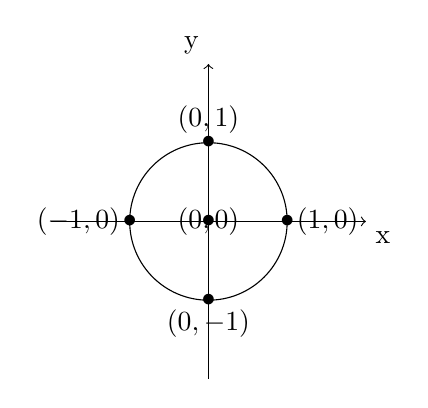
\begin{tikzpicture}
	\pgfmathsetmacro\MAX{2}
	\draw[->] (-\MAX,0) -- (\MAX,0) node[anchor=north west] {x};
	\draw[->] (0,-\MAX) -- (0,\MAX) node[anchor=south east] {y};
	\draw node at (0,0) {$(0,0)$};
	\draw node at (0,0) {$\bullet$};
	\draw node at (0,1) {$\bullet$};
	\draw node at (0,1) [anchor=south]{$(0,1)$};
	\draw node at (1,0) {$\bullet$};
	\draw node at (1,0) [anchor=west] {$(1,0)$};
	\draw node at (-1,0) {$\bullet$};
	\draw node at (-1,0) [anchor=east] {$(-1,0)$};
	\draw node at (0,-1) {$\bullet$};
	\draw node at (0,-1) [anchor=north]{$(0,-1)$};
	\draw (0,0) circle (1);
	\end{tikzpicture}\\
	Per prima cosa osservo che s possono trovare dei punti che rendono vera $f(x,y)=x^2+y^2-1=0$ e sono tutti i punti della circonferenza di centro l'origine degli assi e raggio unitario.\\
	il punto $(x_0,y_0)=(0,1)$ definisce implicitamente una funzione $y=\varphi(x)=\sqrt{1-x^2}$ con $\mathcal{X}=[-1,1]$ e $\mathcal{Y}=[0,1]$\\
	un primo problema è dovuto alla scelta degli intervalli $\mathcal{X},\mathcal{Y}$, per esempio posso scegliere $\mathcal{X}=[-\frac{1}{2},\frac{1}{2}]$ e $\mathcal{Y}=R^+$\\
	un secondo problema è la scelta del punto $(x_0,y_0)$, potrei scegliere il punto $(\frac{1}{\sqrt{2}},\frac{1}{\sqrt{2}})$\\
\observation
La stessa definizione può essere riscritta con la $x$ funzione della $y$ poiché a priori non c'è distinzione tra le variabili.
\proposition (caso lineare)\\
sia $f:R^n\times \R^m\rightarrow \R^p$ che $(x,y)\rightarrow Ax+By-C$ con $A\in Mat(p \times n), B\in (p \times m), B\in (p \times 1)$. Se $p=m$ cioè $B$ è un matrice quadrata, e $det(B)\ne 0$ cioè invertibile, allora\\
$\exists !\varphi : \R^n\rightarrow \R^m$ t.c.: $f(x,y)=0 \iff y=\varphi(x)$
\begin{proof}
	$f(x,y)=0\iff Ax+By=-C\iff By=-Ax+C\iff y=-B^{-1}Ax+B^{-1}C = \varphi(x)$
\end{proof}
\begin{theorem}[Teorema della Funzione Implicita]
	\label{teo:funz_impl}
	Sia $f:X\times Y\rightarrow \R^m$ con $X\subseteq \R^n, Y\subseteq \R^m$\\
	Preso un punto $(x_0,y_0)$ con $x_0\in \circdot{X}$,$y_0\in \circdot{Y}$\\
	se:
	\begin{enumerate}
		\item $f$ continua in $X\times Y$
		\item $f(x_0,y_0)=0$
		\item $f$ differenziabile rispetto a $y \forall (x,y)\in X\times Y$ e $D_yf(x,y)$ continua.
		\item $D_yf(x_0,y_0)$ invertibile .
	\end{enumerate}
	$\Rightarrow $ si ha:\\
	esistenza della funzione implicita\\
	$\exists \mathcal{X}\subseteq X$ intorno di $x_0$(xstrano aperto)\\
	$\exists \mathcal{Y}\subseteq Y$ intorno di $y_0$(ystrano aperto)\\
	$\exists\varphi$ continua con $\varphi:\mathcal{X}\rightarrow\mathcal{Y}$ t.c. $[\varphi (x_0)=y_0 e] f(x,y)=0, x\in\mathcal{X},y\in\mathcal{Y} \iff y=\varphi(x)$
	unicità di sostanza cioè a meno del dominio:\\
	se $\varphi_i:\mathcal{X}_i\rightarrow\mathcal{Y}_i$ e $x_0\in\mathcal{X}_i,y_0\in\mathcal{Y}_i$\\
	$f(x_0,y_0)=0 \forall x\in\mathcal{X}_i, y\in \mathcal{Y}\iff y=\varphi_i(x)$ con $i=1,2$\\
	Allora $\forall\in\mathcal{X}\cap\mathcal{X}_1\cap\mathcal{X}_2$ vale $\varphi_1(x)=\varphi_2(x)$

	\observation
	Le ipotesi 3 e 4 garantiscono che esiste una approssimazione lineare, l'ipotesi 4 è sensata poiché $y$ e $f$ hanno lo stesso numero di componenti quindi $Dyf$ è un matrice qudrata.\\
	la funzione $f:X\times Y\rightarrow \R^m$ che $(x,y)\rightarrow f(x,y)$ ??????\\
	cioè $\forall x\in X$ (sto fissando una x) $f^x:Y\rightarrow \R^m$ che $y\rightarrow f(x,y)$(sto variando la y), $Df^x\in Mat(m\times m)$

	\observation Metodo degli zeri di Newton per troare gli zeri di una funzione o metofo delle tangenti.\\
	\resizebox {\columnwidth} {!} {
	\begin{tikzpicture}
	\draw[->] (-1,0) -- (5,0) node[anchor=north west] {y};
	\draw[->] (0,-1) -- (0,4) node[anchor=south east] {z};
	\draw[domain=-1:4,smooth,variable=\x,blue] plot ({\x},{(1/8)*(\x*\x)-(\x)+1.9});
	\end{tikzpicture}
	}\\
	Scelgo un punto $y_0$ ne prendo il valore sulla curva, disegno la tangente e chiamo $y_1$ l'intersezione con l'asse $y$. Itero il processo $y_n+1=y_n\frac{f(y_n)}{f'(y_n)}$\\
	discorso al momento difficile per me....\\
	\begin{proof}
		Dobbiamo partire da $f(x,y)=0$ arrivare a $y=\varphi(x)$,vogliamo applicare un raginamento simile a quello della Metodo di Newton, passando però per il concetto di punto fisso, il teorema delle Contrazioni ci assicura che esiste unico.\\
		cerchiamo quindi una contrazione $T$ il cui punto fisso sia soluzione di $f(x,y)=0$. $T$ è del tipo:\\
		$T:?\times ?\rightarrow ?$\\
		$(x,y)\rightarrow y-[D_yf(X_0,y_0)]^{-1}f(x,y)$, nota che non avere nella derivata lo stesso punto in cui si calcola la funzione (come è nel metodo di Newton) ha effetti "tragici" sulla velocità di convergenza, ma a noi interessa l'esistenza.\\
		bisgna capire quali insiemi usare come insiemi di partenza e arrivo, devo essere scelti in modo da poter applicare il teoremma delle contrazioni. Bisogna scegliere sottoinsiemi di $R^n$ e $R^m$, scegliamo quindi delle sfere\\
		$T:\overline{B(x_0,r_x)}\times\overline{B(y_0,r_y)}\rightarrow\overline{B(y_0,r_y)}$, scegliendo la chiusura delle sfere si è sicuri di lavorare in uno spazio metrico completo, poiché in $R^l$ completo $\iff$ chiuso e limitato.\\
		come vengono invece scelti i raggi? sono scelti in modo che:\\
		\begin{enumerate}
			\item $T$ è ben definita
			\item $\forall x \in \overline{B(x_0,r_x)} Tx: \overline{B(x_0,r_x)}\rightarrow\overline{B(y_0,r_y)}$ che $y\rightarrow T(x,y)$,\\
		\end{enumerate}
		cioè $T$ è una contrazione tale che $\forall x$ esiste un punto fisso, $\forall x$ associo a $y$ una x, e quindi na funzione.\\
		$r_x,r_y$ devono essere sufficientemente piccoli per avere tali proprietà e per poterci lavorare sopra.\\
		Abbiamo che $f(x,y)=0 \iff T(x,y)=y$\\
		$T(x,y)=y\iff y=y-[D_yF(x_0,y_0)]^{-1}f(x,y)$\\
		$[D_yF(x_0,y_0)]^{-1}f(x,y)\iff f(x,y)=0$\\
		Per verificare che $T$ è una contrazione ne stimo la norma\\
		$\norm{T(x,y_2)-T(x,y_1)} \le \sup\limits_{\widetilde{y}\in segmento}\norm{D_yT(x,\widetilde{y})}\norm{y_2-y_1} $  accrescimenti finiti.\\
		Poichè le sfere sono insiemi convessi è stato possibile applicare il Teorema degli accresscimenti finiti.\\
		Presa $T(x,y) = y-[D_yf(x_0,y_0)]^{-1}f(x,y)$, la derivo rispetto a $y$:
		\[D_yT(x,y)= I_\R^m-[D_yf(x_0,y_0)]^{-1}D_yf(x,y) = \]
		\[=[D_yf(x_0,y_0)]^{-1}][D_yf(x_0,y_0)-D_yf(x,y)]\]
		Osserviamo che abbiamo ottenuto una matrice come costante moltiplicativa, al secondo membro abbiamo la differenza di due valori di una funzione, che per ipotesi è una funzione continua ($D_yf(x,y)$ continua), allora per $r_x$ e $r_y$ sufficientemente piccoli ho che:\\
		$\norm{D_yT(x,y)} \le \frac{1}{2}$, è scelto questo valore poiché è comodo al fine di dimostrare la contrazione...\\
		\[\norm{D_yT(x,y)} \le \norm{D_yf(x_0,y_0)]^{-1}} \norm{D_yf(x_0,y_0)-D_yf(x,y)}\le\frac{1}{2} \]  
		\[\norm{T(x,y_2)-T(x,y_1)}\le\frac{1}{2}\norm{y_2-y_1} \]
		Se dimostriamo che $T$ è ben definita abbiamo dimostrato che $T$ è una contrazione.\\
		Per verificare che $T$ è en definita bisogna mostrare che $T(x,y)\subseteq\overline{B(y_0,r_y)}$ quindi si mostra che la distanza tra $T(x,y)$ e il centro è minore di $r_y$
		\[\norm{T(x,y) - y_0}\le\norm{T(x,y)-T(x,y_0)}+\norm{T(x,y_0)-y_0} \le\]
		\[\le\frac{1}{2}\norm{y-y_0}+\norm{y_0-[D_yf(x_0,y_0)]^{-1}f(x,y_0)-y_0}\le\]
		\[\le\frac{1}{2}\norm{y-y_0}+\norm{[D_yf(x_0,y_0)]^{-1}} \norm{f(x,y_0)-0}\le\]
		\[\le\frac{1}{2}\norm{y-y_0}+\norm{[D_yf(x_0,y_0)]^{-1}} \norm{f(x,y_0)-f(x_0,y_0)}\le\]
		\[\le\frac{1}{2}r_y+\frac{1}{2}r_y\le r_y\]
		Allora $T$ è ben definita perché $T(x,y)\in\overline{B(y_0,r_y)}$.\\
		In conclusione con $\mathcal{X}=\overline{B(x_0,r_x)}$ e $\mathcal{Y}=\overline{B(y_0,r_y)}$ ho che $T:\mathcal{X}\times\mathcal{Y}\rightarrow\mathcal{Y}$ è tale che $\forall x\in\mathcal{X}$ la funzione $y\rightarrow T(x,y)$ è una contrazione e $\overline{B(y_0,r_y)}$ è completo.\\
		quaolcosa sui completi.........\\
		................................\\
		..........................\\
		A questo punto può essere applicato il teorema delle contrazioni:\\
		$\forall x \in \mathcal{X}, \exists y \in\mathcal{Y}: f(x,y)=0$ allora chiamo $\varphi:\mathcal{X}\rightarrow\mathcal{Y}$ che $x\rightarrow y$ è unica quindi $\varphi$ è una funzione.\\
		Allora la funzione implicita esiste. La continuità direva direttamente dal teorema delle contrazioni: l'applicazione che al parametro associa il punto fisso è continua.\\
		Per l'unicità si osservano le ipotesi 1 e 2, dove è scritto $\forall x$ ovvero scelta una qualunque $x$ la $y$ è unica quindi $\varphi$ è univocamente definita.
		
	\end{proof}
\end{theorem}
\proposition
Sia $f:X\times Y\rightarrow \R^m$ con $X\in \R^n, Y\in \R^m$\\
Preso un punto $(x_0,y_0)$ con $x_0\in \circdot{X}$,$y_0\in \circdot{Y}$\\
se:
\begin{enumerate}
	\item $f(x_0,y_0)=0$
	\item $f\in \cntclass{1}(X\times Y,R^m)$.
	\item $D_yf(x_0,y_0)$ invertibile .
\end{enumerate}
$\Rightarrow $ si ha:\\
\begin{enumerate}
	\item $\exists \varphi: \mathcal{X}\rightarrow\mathcal{Y}$ definita implicitamente da $f(x_0,y_0)=0$
	\item $\varphi$ continua su $\mathcal{X}$
	\item $\varphi$ è differenziabile e $D\varphi(x)=-[D_yf(x,\varphi(x))]^{-1}D_xf(x,\varphi(x))$
\end{enumerate}
\begin{proof}
	I punti 1 e 2 sono gli stessi del teorema della funzione implicita e si dimostrano allo stesso modo.\\
	Per il punto 3 abbiamo che $f(x,y)=0\iff y=\varphi(x)$ e quindi $\forall x\in \mathcal{X}$ $f(x,\varphi(x))=0$\\
	.........\\
	.........\\
	
\end{proof}

\proposition CASO N=1, M=1\\
Sia $f:X\times Y\rightarrow \R$ con $X\in \R, Y\in \R$\\
Preso un punto $(x_0,y_0)$ con $x_0\in \circdot{X}$,$y_0\in \circdot{Y}$\\
se:
\begin{enumerate}
	\item $f(x_0,y_0)=0$
	\item $f\in \cntclass{1}(X\times Y,R)$.
	\item $\partial_yf(x_0,y_0)\ne 0$.
\end{enumerate}
$\Rightarrow $ si ha:\\
\begin{enumerate}
	\item $\exists \varphi: \mathcal{X}\rightarrow\mathcal{Y}$ definita implicitamente da $f(x_0,y_0)=0$
	\item $\varphi\in \cntclass{0}(\mathcal{X},\mathcal{Y})$
	\item $\varphi$ è derivabile e $\varphi'(x)=-[\partial_yf(x,\varphi(x))]^{-1}\partial_xf(x,\varphi(x))$
\end{enumerate}
\begin{proof}
	$f(x,y)=0\iff y=\varphi(x)$, derivando $D(f(x,\varphi(x)))=0$\\
	$\partial_xf(x,\varphi(x))+\partial_yf(x,\varphi(x))\varphi'(x)=0$\\
	allora $\varphi'(x) = -\frac{\partial_xf(x,\varphi(x))}{\partial_yf(x,\varphi(x))}$
\end{proof}
\observation Non essendoci motivo per preferire la $x$ alla $y$ o viceversa, esiste anche una versione di questo teorema  in  cui le ipotesi sono le stesse eccetto l'ultima che diventa $\partial_xf(x_0,y_0)\ne 0$
\begin{enumerate}
	\item $\exists \psi: \mathcal{Y}\rightarrow\mathcal{X}$ definita implicitamente da $f(x,y)=0$
	\item $\psi\in \cntclass{0}(\mathcal{Y},\mathcal{X})$
	\item $\psi$ è derivabile e $\psi'(y)=-[\partial_xf(\psi(y),y)]^{-1}\partial_yf(\psi(y),y)$
\end{enumerate}
Qualche esempio qui\\
\subsection{Il Teorema della funzione Inversa}
Data una funzione f, poterla invertire  ...... unico modo l'equazione (o sistema ....)... l'incognita $x$ in funzione del parametro .....\\
\proposition(Teorema della funzione inversa caso lineare)\\
Sia $f:R^n\in \R^m$ data da $f(x)=Mx$ e $M\in Mat(m\times n)$, $f$ è invertibile $\iff n=m$ e $detM\ne 0$
\proposition(caso generale)\\
sia $f:A\rightarrow \R^n$ con $A\in \R^n$, $f\in \cntclass{1}(A,R^n)$, $x_0\in \circdot{A}$ e $Df(x_0)$ invertibile.\\
Allora $\exists\mathcal{X}\in A,\exists\mathcal{Y}\in \R^n$, $\exists\varphi\mathcal{Y}\rightarrow\mathcal{X}$ con la proprietà $f(x)=y\iff x=\varphi(y)$ con $x\in\circdot{\mathcal{X}}$ e $y\in\circdot{\mathcal{Y}}$ e $\varphi\in \cntclass{1}(\mathcal{Y},\mathcal{X})$ e $D\varphi(y)=[Df(x)]^{-1}$\\
\begin{proof}
	$f(x)=y\iff f(x)-y=0$. Allora introduco $F:A\times \R^n\rightarrow \R^n$ data da $F(x,y)=f(x)-y$.\\
	Studio $F(x,y)=0$ per ottenere $x=\varphi(y)$.\\
	Per poter applicare il teorema della funzione implicita serve $D_xF(x_0,y_0)$ invertibile, ma $D_xF(x_0,y_0)=Df(x_0)$ che è invertibile per ipotesi.\\
	Applico allora il teorema della funzione implicita , quindi gli intorni esistono e $x=\varphi(y)$.\\
	resta da trovare la derivata totale di $\varphi$. Sappiamo che $f\in \cntclass{1}$ quindi $\varphi \in \cntclass{1}$.\\
	Sappiamo che $\varphi(f(x))=x$, applicando la derivata della funzione composta abbiamo che:\\
	$D\varphi(f(x))Df(x)=I$\\
	$D\varphi=[Df(x)]^{-1}$ quando $\varphi(y)=x$\\
	si puo anche scrivere come $(Df^{-1})(f(x))=[Df(x)]^{-1}$
\end{proof}
\section{Massimi e Minimi Liberi}
\definition
Siano $(X,d)$s.m., $A\subseteq X$ e $f:A\rightarrow \R$, siano $x_0\in A, B\in A$ e $m,M\in \R$ ( L'insieme immagini deve essere $R$ per poter parlare di massimi e minimi, $R$ è un campo ordinato a differenza di $R^n$).\\
$M$ è massimo di $f$ su $B \bydef M=\max f(B)\iff\forall x \in B f(x_0)\ge f(x)$\\
$M$ è minimo di $f$ su $B \bydef m=\min f(B)\iff\forall x \in B f(x_0)\le f(x)$\\
$x_0$ è punto di massimo assoluto per $f \bydef f(x_0)=\max\limits_{A}f(x)$\\
$x_0$ è punto di minimo assoluto per $f \bydef f(x_0)=\min\limits_{A}f(x)$\\
$x_0$ è punto di massimo locale relativo per $f \bydef \exists r>0: f(x_0)=\max\limits_{x\in B(x_0,r)}f(x)$ con $B(x_0,r)\subseteq A$\\
$x_0$ è punto di minimo locale relativo per $f \bydef \exists r>0: f(x_0)=\min\limits_{x\in B(x_0,r)}f(x)$ con $B(x_0,r)\subseteq A$\\
\subsection{Condizioni Necessarie}
\proposition{Teorema di Fermat}\\
sia $f:A\subseteq \R^n\rightarrow \R$ e $x_0\in\circdot{A}$. Se $x_0$ è punto di massimo(0 minimo) locale per $f$ su $A$ e $f$ è differenziabile in $x_0$ allora $\nabla f(x_0)=0$.
\begin{proof}
	Sia $v\in \R^n$ con $\norm{v} =1$, la funzione $F(t)= f(x_0+tv)$ che a $t\rightarrow x_0+tv$ è il moto rettilineo uniforme che passa da $x_0$ all'istante $0$ e si muove con velocità vettore costante $v$. cioè per tempi negativi mi avvicino a $x_0$ al tempo zero si è in $x_0$ e per tempi positivi si allontana da $x_0$. quindi $t=0$ è punto di massimo per $F$, allora $F'(0) = 0$ per il teorema di Fermat di A1.\\
	Ora abbiamo che $F'(t)=\nabla f(x_0+tv)v$ quindi $F'(0)=\nabla f(x_0)v$ cioè $\nabla f(x_0)v=0$.\\
	Quindi $\forall v :\norm{v} =1$ vale $\nabla f(x_0)=0$\\
	OSS:: Vale anche che $D_vf(x_0)=0$
\end{proof}
\definition
sia $f:A\subseteq r^n\rightarrow \R$, $x_0\in\circdot{A}$\\
$x_0$ è punto stazionario .... $\bydef$ $f$ è differenziabile in $x_0$ e $\nabla f($ ......
\observation
nel caso $n=2, m=1, \nabla f(x_0,y_0)=[\partial_xf(x_0,y_0), \partial_yf(x_0,y_0)]$ ..... i punti stazionari sono quelli che ......parziali.
\observation
Prima di continuare un paio di osservazioni sulle forme quadratiche.\\
\definition
forma quadratica su $R^n \bydef q:R^n\rightarrow \R$ che $x\rightarrow x^TQx$ con $Q\in Mat(n\times n)$ simmetrica\\
ESEMPI:n=2\\
\[
Q=\begin{bmatrix}1&&0\\0&&1\end{bmatrix}\quad
Q=\begin{bmatrix}-1&&0\\0&&-1\end{bmatrix}\quad
Q=\begin{bmatrix}-1&&0\\0&&1\end{bmatrix}\quad 
\]
SEMPRE POSITIVA SEMPRE NEGATIVA CAMBIA SEGNO\\
SEMPRE POSITIVA SEMPRE NEGATIVA CAMBIA SEGNO\\
SEMPRE POSITIVA SEMPRE NEGATIVA CAMBIA SEGNO\\
\proposition
se $Q$ è una forma quadratica, allora\\
\begin{itemize}
	\item $\forall\lambda\in \R, \forall x\in \R^n$ $q(\lambda x)=\lambda^2q(x)$
	\item $q(0)=0$
	\item se $q$ è limitata $\Rightarrow q\equiv 0$ 
\end{itemize}
\begin{proof}
	\begin{itemize}
		\item $q(\lambda x)=(\lambda x)^TQ(\lambda x)=\lambda^2x^TQx=\lambda^2q(x)$
		\item $q(0)=q(0x)=0q(x)=0$
		\item (contronominale $q\ne 0 \Rightarrow q$ non è limitata).\\
		se $q$ è non nulla $\Rightarrow \exists x \in \R^n$ $q(x)\ne 0$\\
		allora $q(\lambda x)=\lambda^2q(x)$ illimitata.
		\item ???????????????????????????????????????????????
	\end{itemize}
\end{proof}
\proposition
se $q$ è una forma quadratica $\Rightarrow\exists M\ge 0: \abs{q(x)}\le M\norm{x}^2$ $\forall x\in \R^n$
\begin{proof}
	per $x\ne 0$ $\abs{q(x)} =\abs{q\left(\norm{x} \frac{1}{\norm{x} }x\right)} = \norm{x}^2\abs{q\left(\frac{1}{\norm{x}}x\right)}\le$\\
	$\le\left(\sup\limits_{\norm{x}=1}\abs{q(x)}\right)\norm{x}^2=\le\left(\max\limits_{\norm{x}=1}\abs{q(x)}\right)\norm{x}^2=M\norm{x}^2$
\end{proof}
\proposition
Sia $q$ una forma quadratica, se $q(x)=o(\norm{x}^2)$ per $x\rightarrow 0 \Rightarrow q\equiv 0$
\begin{proof}
	sia $x\in \R^n$ con $\norm{x}=1$ e $t>0$.\\
	$q(x)=\frac{1}{t^2}$, $q(tx)=\frac{q(tx)}{\norm{tx}^2}\rightarrow 0$ per $t\rightarrow 0$ per ipotesi.\\
	Allora $\forall x$ con $\norm{x}$ vale $q(x)=0$ e allora $\forall x\ne 0, q(x)=q\left(\frac{1}{\norm{x}}x\right)\norm{x}^2$
\end{proof}
\definition
Sia $q:R^n\rightarrow \R$ una forma quadratica\\
\begin{itemize}
	\item $q$ è definita positiva $\bydef \forall x\in \R^n, x\ne 0$ $q(x)>0 [Q>0]$
	\item $q$ è semidefinita positiva $\bydef \forall x\in \R^n$ $q(x)\ge0 [Q\ge0]$
	\item $q$ è definita negativa $\bydef \forall x\in \R^n, x\ne 0$ $q(x)<0 [Q><0]$
	\item $q$ è semidefinita negativa $\bydef \forall x\in \R^n$ $q(x)\le0 [Q\le0]$
\end{itemize}
\proposition
Sia $q:R^n\rightarrow \R$ una forma quadratica, se $q$ è definita positiva $\Rightarrow \exists m>0: \forall x \in \R^n, q(x)\ge m\norm{x}^2$
\begin{proof}
	Noto che $q(\lambda x)=\lambda^2q(x)$\\
	$q(x)=q\left(\frac{1}{\norm{x}}x\norm{x}^2\right)\ge\min\limits_{\norm{x}=1}q(\lambda)\norm{x}^2$
\end{proof}
Ora dobbiamo cercare di capire se $q$ è definita positiva\\
Ad esempio: $Q=\begin{bmatrix}1&&0&&0\\0&&-1&&0\\0&&0&&0\end{bmatrix}$ è facile capire che è semodefinita positiva poiché è in diagonale, quindi la prima cosa da fare è trovare una forma diagonale per $Q$\\
un procedimento pratico e veloce è il seguente:\\
\[Q=\begin{bmatrix}q_{11}&&q_{12}&&q_{13}&&\ldots\\q_{21}&&q_{22}&&q_{23}&&\ldots\\q_{31}&&q_{32}&&q_{33}&&\ldots\\\vdots&&\vdots&&\vdots&&\ddots\end{bmatrix}\rightarrow\begin{bmatrix}\lambda_{1}&&0&&0&&\ldots\\0&&\lambda_{2}&&0&&\ldots\\0&&0&&\lambda_{3}&&\ldots\\\vdots&&\vdots&&\vdots&&\ddots\end{bmatrix}\]
\[\lambda=q_{11},\quad\lambda_{2}=\frac{detQ_2}{q_11}\quad\lambda_{3}=\frac{detQ_3}{detQ_2}\quad ...\quad \lambda_{i}=\frac{detQ_i}{detQ_{i-1}}\]
Questo perché se dobbiamo valutare il segno dell'incremento della f ci servono le variazioni sulle quadriche. Se $f$ è $\cntclass{2}$ scrivo lo sviluppo di Taylor al secondo ordine:\\
\[f(x)-f(x_0)=\nabla f(x_0)(x-x_0)+\frac{1}{2}(x-x_0)^TH_f(x_0)(x-x_0)+o(\norm{x-x_0}^2)\]
max e min dove $\nabla f(x_0)=0$ per Fermat, l'o piccolo è trascurabile, allora il segno della derivata dipende dalla forma quadratica al secondo membro.
\proposition
sia $f:A\subseteq \R^n\rightarrow \R$ e $x_0\in\circdot{A}$.\\
$f\in \cntclass{2}(A;R)$ e $x_0$ punto di massimo locale per $f$ su $A\Rightarrow\nabla f(x_0)=0$ e $H_f(x_0)$ è semidefinita negativa.
\begin{proof}
	$f(x)-f(x_0)=\frac{1}{2}(x-x_0)^TH_f(x_0)(x-x_0)+o(\norm{x-x_0}^2)$ poiché $f\in \cntclass{2}$\\
	il primo termine è negativo poiché per ipotesi $x_0$ è punto di massimo locale, ne segue che il termine $(x-x_0)^TH_f(x_0)(x-x_0)$ non può essere positivo. 
\end{proof} 
\proposition
sia $f:A\subseteq \R^n\rightarrow \R$ e $x_0\in\circdot{A}$.\\
$f\in \cntclass{2}(A;R)$ e $x_0$ punto di minimo locale per $f$ su $A\Rightarrow\nabla f(x_0)=0$ e $H_f(x_0)$ è semidefinita positiva.
\begin{proof}
	$f(x)-f(x_0)=\frac{1}{2}(x-x_0)^TH_f(x-x_0)+o(\norm{x-x_0}^2)$ poiché $f\in \cntclass{2}$\\
	il primo termine è positivo poiché per ipotesi $x_0$ è punto di minimo locale, ne segue che il termine $(x-x_0)^TH_f(x-x_0)$ non può essere negativo. 
\end{proof} 


\subsection{Condizioni Sufficienti}
\proposition
sia $f:A\subseteq \R^n\rightarrow \R$ e $x_0\in\circdot{A}$.\\
$f\in \cntclass{2}(A;R)$, $\nabla f(x_0)=0$,$H_f(X_0)$ è definita negativa $\Rightarrow x_0$ è un punto di massimo locale per $f$
\begin{proof}
	$f\in \cntclass{2}$ quindi possiamo scrivere:\\
	$f(x_+h)-f(x_0)=\nabla f(x_0)h+\frac{1}{2}(h)^TH_f(x_0)+o(\norm{h}^2)$ per $h\rightarrow 0$\\
	$f(x_+h)-f(x_0)=\frac{1}{2}(h)^TH_f(x_0)+o(\norm{h}^2)$ per $h\rightarrow 0$\\
	Sappiamo che $H_f$ è definita negativa per ipotesi, allora $h^TH_f(x_0)h\le -m\norm{x_0}$ allora $f(x_0+h)-f(x_0)<0$ e quindi $x_0$ è punto di massimo locale per $f$.
\end{proof} 
\proposition
sia $f:A\subseteq \R^n\rightarrow \R$ e $x_0\in\circdot{A}$.\\
$f\in \cntclass{2}(A;R)$, $\nabla f(x_0)=0$,$H_f(X_0)$ è definita positiva $\Rightarrow x_0$ è un punto di minimo locale per $f$
\begin{proof}
	$f\in \cntclass{2}$ quindi possiamo scrivere:\\
	$f(x_+h)-f(x_0)=\nabla f(x_0)h+\frac{1}{2}(h)^TH_f(x_0)+o(\norm{h}^2)$ per $h\rightarrow 0$\\
	...........\\
	...........\\
\end{proof} 
QUALCHE DISEGNO E SPIEGAZIONE.....
\subsection{Il Significato Geometrico del Gradiente n=2 m=1}
\definition
Sia $A\subseteq \R^2$ e $f:A\rightarrow \R$\\
La suferficie $z=f(x,y)$ è il grafico di $f$, è unsottoinsieme di $R^3$\\
Se $c\in \R$, la curva di livello $c$ di $f$ è l'insieme $f^{-1}(c)\{(x,y)\in A: f(x,y)=c\}$\\
Se $f$ 	'e differenziabile in $(x_0,y_0)\in\circdot{A}$ il piano tangente alla superficie $z=f(x,y)$ in $(x_0,y_0)$ ha equazione:\\
\[z=f(x_0,y_0)+\nabla f(x_0,y_0)\begin{bmatrix}(x-x0)\\(y-y_0)\end{bmatrix}\] 
\[z=f(x_0,y_0)+\partial_xf(x_0,y_0)(x-x_0)+\partial_yf(x_0,y_0)(y-y_0)\]
\observation
geometricamente, il gradiente di una funzione indica la direzione di $R^n$ in cui si ha la massima variazione del valore di f, nel verso di incremento positivo di $f$,
\observation 
osservazione col grafico che al momento non faccio.
\proposition
Siano $A\subseteq \R^n, f:A\rightarrow \R$ differenziabile in $(x_0,y_0)\in \circdot{A}$, l'incremento di $f(x_0+h,y_0+k)-f(x_0,y_0)$ è massimo quando $[h k]=\lambda\nabla f(x_0,y_0)$ con $\lambda >0$ ed è minimo con $[h k]=\lambda\nabla f(x_0,y_0)$ con $\lambda <0$
\begin{proof}
	so che posso approssimare la funzione quindi posso scrivere:\\
	$f(x_0+h,y_0+k)-f(x_0,y_0)=\nabla f(x_0,y_0)\begin{bmatrix}h\\k\end{bmatrix}+o(\sqrt{h^2+k^2})$=
	$=\norm{\nabla f(x_0,y_0)}\norm{\begin{bmatrix}h k\end{bmatrix}}cos(\theta)+o(\sqrt{h^2+k^2})$\\
	dove $\theta$ è l'angolo tra $\nabla f(x_0,y_0)$ e $[h k]$ per $||[h k]||$ sufficientemente piccola, l'incremento $f(x_0+h,y_0+k)-f(x_0,y_0)$ è massimo se $cos( \theta )=1$ ed è minimo se $cos(\theta )=-1$, da cui la tesi.\\ 
\end{proof}
\proposition
siano $f\in \cntclass{1}(A;R)$ con $A\subseteq \R^2$ e $(x_0,y_0)\in\circdot{A}$ e $\nabla f(x_0,y_0)\ne 0$[cioè stazionario]. Allora $nabla f(x_0,y_0)$ è perpendicolare alla curva di livello passante per .....
\observation
un vettore 1'e perpendicolare a una curva se è perpendicolare alla retta o al vettore tangente alla curva in quel punto.
\begin{proof}
	La curva di livello è $f(x,y)=f(x_0,y_0)$ cioè $f(x,y)-f(x_0,y_0)=0$, per trovare la tangente a questa curva è piu facile se si ha $y=\varphi(x)$\\
	Usiamo quindi il teorema della funzione implicita, mi serve che $\partial_yf(x_0,y_0)\ne 0$, questa condizione non è assicurata dalle ipotesi, per ipotesi il gradiente è non nulla quindi almeno una delle due componenti è non nulla.\\
	Inizio con il caso $\partial_yf(x_0,y_0)\ne 0$.\\
	Il T.F.IMPL. assicura che :\\
	$\exists\mathcal{X},\mathcal{Y}$ con $x_0\in\circdot{\mathcal{X}}, y_0\in\circdot{\mathcal{Y}}$, $\exists\varphi:\mathcal{X}\rightarrow\mathcal{Y}$ t.c.:\\
	$f(x,y)=f(x_0,y_0), x\in\mathcal{X}, y\in\mathcal{Y} \iff y=\varphi(x)$\\
	La retta tangente in $x_0$ a $y=\varphi(x)$ è $y=y_0+\varphi'(x_0)(x-x_0)$\\
	questo vuole dire che un vettore tangente a $y=\varphi(x)$ in $(x_0,y_0)$ è $\begin{bmatrix}1\\\varphi'(x_0)\end{bmatrix}$.\\
	... calcolo il prodotto scalare\\
	\[\nabla f(x_0,y_0)\begin{bmatrix}1\\\varphi'(x_0)\end{bmatrix} = \begin{bmatrix}\partial_x f(x_0,y_0)&&\partial_y f(x_0,y_0)\end{bmatrix}\begin{bmatrix}1\\-\frac{\partial_x f(x_0,y_0)}{\partial_y f(x_0,y_0)}\end{bmatrix} =\] 
	\[=\partial_x f(x_0,y_0) -\partial_y f(x_0,y_0)\frac{\partial_x f(x_0,y_0)}{\partial_y f(x_0,y_0)}=0\]
	Allora il graadiente è perpendicolare alla curva di livello.\\
	Guardiamo ora al caso in cui $\partial_yf(x_0,y_0)= 0$ e $\partial_xf(x_0,y_0)\ne 0$ quindi il gradiente è non nullo.\\
	Applicando lo stesso ragionamento id sopra, solo esplicitando la $x$ in funzione della $y$. Quindi $x=\psi(x)$ e $\psi{'}(y_0)=-\frac{\partial_y f(x_0,y_0)}{\partial_x f(x_0,y_0)}$
\end{proof}

\section{Massimi e Minimi Vincolati}
Spesso la ricerca di punti di massimo o minimo di una funzione $f:A\rightarrow \R, A\subseteq \R^n$ deve essere ristrettaad un sottoinsieme $B\subseteq A$ a causa di eventuali vincoli a cui le variabili indipendenti devono soddisfare. L0insieme $B$ può essere generalmente descritto da una funzione $\varphi :A\rightarrow \R^p$, nel senso che $B=\{x\in A:\varphi (x)\le 0\}$\\
NOTA::: direi n>1 poiché se ho una sola variabile e la vincolo ...??????? booooo .\\
Questo problema è usualmente abbreviato in:
\[\max\limits_{\varphi \le 0}\quad o \quad\min\limits_{\varphi \le 0}\]
può essere affrontato in due passi:\\
\begin{enumerate}
	\item ricerca dei punti di estremo di $f$ interni a $B$, problema gia affrontato.
	\item ricerca dei punti di estremo di $f$ sul bordo di $B$, affrontiamo ora.
\end{enumerate}
Sotto opportune condizioni su $\varphi$, infatti, $\circdot{B} = \{x\in A:\varphi(x)<0\}$ e $\partial B\{x\in A:\varphi(x)=0\}$
\proposition{Teorema dei Moltiplicatori di Lagrange}
Siano $f,g:A\subseteq \R^2\rightarrow \R, (x_0,y_0)\in\circdot{A}, g(x_0,y_0)=0, f,g\in \cntclass{1}(A;R)$, $\nabla g (x_0,y_0)\ne 0$\\
Se $(x_0,y_0)$ è di max(o min) locale per $f$ su $g=0\Rightarrow\exists \lambda in \R$ t.c: $\nabla f(x_0,y_0) = \lambda g(x_0,y_0)$ (all fin fine posso dire che sono paralleli).\\
\observation
$\lambda$ si chiama "moltiplicatore di lagrange"
\observation
Se abbiamo un problema del tipo $\max\limits_{g(x,y)=0}f$ cioè il massimo di $f$ sul vincolo $g(x,y)=0$, ci dobbiamo ricondurre ad un sistema del tipo
$\begin{cases} \nabla f(x_0,y_0)=\lambda \nabla g(x_0,y_0)\\ g(x_0,y_0)=0 \end{cases}=\begin{cases} \partial_xf(x_0,y_0)=\lambda \partial_xg(x_0,y_0)\\\partial_yf(x_0,y_0)=\lambda \partial_yg(x_0,y_0)\\ g(x_0,y_0)=0 \end{cases}$\\
3 equazioni in 3 incognite($x,y,\lambda$)\\
In certi casi si introduce una funzione $\mathcal{L}(x,y,\lambda) = f(x,y)-\lambda g(x,y)$ detta Lagrangiana, i punti stazionari vincolati di $f$ sono punti stazonari liberi della Lagrangiana.\\
\begin{proof}
	Sappiamo che $\nabla g(x_0,y_0)\ne$ quindi $\begin{bmatrix}\partial_xg(x_0,y_0) &&\partial_yg(x_0,y_0)\end{bmatrix}\ne\begin{bmatrix}0&&0\end{bmatrix}$ quindi o $\partial_xg(x_0,y_0)\ne 0$ o $\partial_yg(x_0,y_0)\ne 0$.
	Mettiamoci nel caso in cui $\partial_yg(x_0,y_0)\ne 0$,\\
    Per il teorema della funzione implicita ho che :\\
	$\exists\mathcal{X},\mathcal{Y}$ con $x_0\in\circdot{\mathcal{X}}, y_0\in\circdot{\mathcal{Y}}$, $\exists\varphi:\mathcal{X}\rightarrow\mathcal{Y}$ t.c.:\\
	$g(x,y)=f(x_0,y_0), x\in\mathcal{X}, y\in\mathcal{Y} \iff y=\varphi(x)$\\
	Osserviamo che dire $(x_0,y_0)$ di massimo o minimo per $f$ ristretta a $g(x,y)=0\iff x_0$ è di massimo o di minimo per la funzione $x\rightarrow f(x,\varphi(x))$.\\
	Per il teorema di Fermat $\left.\frac{\mathrm{d}}{\mathrm{d}x}(f(x,\varphi(x)))\right\|_{x=x_0}=0$, punto stazionario ha derivata nulla, e la derivata di quella funzione in $x_0$ è:
	\[\partial_xf(x_0,\varphi(x_0))+\partial_yf(x_0,\varphi(x_0))\cdot\varphi'(x_0)\] 
	allora
	\[0=\partial_xf(x_0,\varphi(x_0))+\partial_yf(x_0,\varphi(x_0))\cdot\varphi'(x_0)=\]
	\[=\partial_xf(x_0,\varphi(x_0))-\partial_yf(x_0,\varphi(x_0))\frac{\partial_xg(x_0,\varphi(x_0))}{\partial_yg(x_0,\varphi(x_0))}=\]\\
	\[=\partial_xf(x_0,\varphi(x_0))\partial_yg(x_0,\varphi(x_0))-\partial_yf(x_0,\varphi(x_0))\partial_xg(x_0,\varphi(x_0))=det\left(\begin{matrix}\partial_xf(x_0,y_0)&&\partial_yf(x_0,y_0)\\\partial_xg(x_0,y_0)&&\partial_yg(x_0,y_0)\end{matrix}\right)=0\]\\
	questo equivale a dire che i vettori riga della matrice sono paralleli quindi $\exists\alpha\in \R : \nabla f(x_0,y_0)=\lambda\nabla g(x_0,y_0)$.\\
	Non è uguale scrivere $\exists\alpha\in \R : \nabla g(x_0,y_0)=\lambda\nabla f(x_0,y_0)$ poiché non c'è certezza sul valore di $\nabla f(x_0,y_0)$ che se nullo negherebbe l'ipotesi di $\nabla g(x_0,y_0)\ne 0$\\
	Se guardiamo ora il caso in cui $\partial_yg(x_0,y_0)=0$ e $\partial_xg(x_0,y_0)\ne 0$.\\
	Seguendo un ragionamento analogo si esplicita $x=\psi(y)$ così che cercare max(o min) di $f$ ristretta a $g(x,y)=0$ porti a $y\rightarrow f(\psi(y),y)$ 
\end{proof}
\proposition{Teorema dei Moltiplicatori di Lagrange caso generale}
Sia $A\in \R^n$, $f\in \cntclass{1}(A;R)$, $g\in \cntclass{1}(A;R^p)$ con $p<n$(n.vincoli<n.variabili), sia poi $x_0\in\circdot{A}, g(x_0)=0, Dg (x_0,y_0)$ di rango $p$.\\
Se $x_0$ è di max(o min) locale per $f$ su $g=0\Rightarrow\exists \lambda_1,\ldots,\lambda_p in \R$ t.c: $\nabla f(x_0,y_0) = \sum\limits_{i=1}^{p}\lambda_i\nabla g(x_0,y_0)$\\
\section{Il caso \texorpdfstring{$n=2,\,m=1$}{n=2, m=1}}
%TODO This section is a placeholder
\section{Derivate e Integrali}
\begin{proposition}[Teorema Fondamentale del Calcolo Integrale]
	\label{teo:fondament_calcolo_integ}
	Sia $I\subseteq \R$ un intervallo e sia $x_0\in I$. Data $f\in c^0(I;R)$ la funzione:
	\[\begin{array}{rcl} F: I & \to & \R \\ x & \to & \int_{x_0}^{x}f(t)\integrald{t} \end{array}\]
	Si ha $F\in \cntclass{1}(I;R)$ e $F'(x)=f(x)$ $\forall x \in I$
\end{proposition}[]
\proposition
Sia $A\subseteq \R^n$ un aperto, data $f\in \cntclass{0}(A\times \R;R)$ la funzione \\
$\begin{array}{rcl} F: \R\times \R\times A & \to & \R \\ (\alpha,\beta,x) & \to & \int_{\alpha}^{\beta}f(x,t)\integrald{t} \end{array}$\\
è di classe $\cntclass{0}(R\times \R\times A;R)$
\proposition
Sia $A\subseteq \R^n$ un aperto, data $f\in \cntclass{1}(A\times \R;R)$ la funzione \\
$\begin{array}{rcl} F: \R\times \R\times A & \to & \R \\ (\alpha,\beta,x) & \to & \int_{\alpha}^{\beta}f(x,t)\integrald{t} \end{array}$\\
è di classe $\cntclass{1}(R\times \R\times A;R)$ ed inoltre, $\forall (\alpha,\beta,x)\in \R\times \R\times A$ e $\forall i=1,\ldots,n$\\
\[\frac{\partial F}{\partial \alpha}=-f(x,\alpha)\]
\[\frac{\partial F}{\partial \beta}=f(x,\beta)\]
\[\frac{\partial F}{\partial x_i}=\int_{\alpha}^{\beta}\frac{\partial F}{\partial x_i}(x,t)\integrald{t}\]
\[\nabla F=\int_{\alpha}^{\beta}\nabla f(x,t)\integrald{t}\]
\corollary
Sia $A\subseteq \R^n$ un aperto, date le funzioni $\alpha:x\rightarrow \R, \beta:x\rightarrow \R, f:x\rightarrow \R, $ di classe $\cntclass{1}$ , la funzione \\
$\begin{array}{rcl} F: A & \to & \R \\ (x) & \to & \int_{\alpha(x)}^{\beta(x)}f(x,t)\integrald{t} \end{array}$\\
è di classe $\cntclass{1}(R\times \R\times A;R)$ ed inoltre, $\forall x_0 \in A$:
\[\nabla F(x_0,y_0)=f(x_0,\beta)\nabla\beta(x_0)-f(x_0,\alpha)\nabla\alpha(x_0)+\int_{\alpha(x_0)}^{\beta(x_0)}\nabla f(x,t)\integrald{t}\]

\section{Funzioni a Valori in \texorpdfstring{$\protect\C$}{C}}
\label{sec:fun_in_C}
Sia $A \subseteq \R^n$ non vuoto. Ogni funzione $A \mapsto \C$ può essere identificata in modo naturale con una funzione $A \mapsto \R^2$ e viceversa.ù
\begin{note}
	Quindi è possibile rappresentare una funzione $A \mapsto \C$ in un piano, detto \textbf{piano complesso} o \textbf{piano di Gauss}
\end{note}
\begin{exercise}
	\label{ex:ext_def_in_C}
	Utilizzando questa identificazione, estendere al caso di funzioni $A \mapsto \C$ le definizioni di continuità, derivabilità, differenziabilità e degli spazi $\cntclass{k}$ date per funzioni $A \mapsto \R$
	% TODO solution
\end{exercise}
\begin{proposition}
	\label{prop:fg_in_C}
	Sia $A \subseteq \R$ e sia $t_0 \in \circdot{A}$. Allora
	\begin{itemize}
		\item Se due funzioni $f,g: A \mapsto \C$ sono differenziabili in $t_0$, anche le funzioni $f+g$ e $f \cdot g$ sono differenziabili in $t_0$. Inoltre
			\[(f+g)'(t_0) = f'(t_0) + g'(t_0) \qquad\text{e}\qquad (f \cdot g)'(t_0) = f'(t_0)g(t_0)+f(t_0)g'(t_0)\]
		\item Per ogni $\lambda \in \C$, anche $\lambda f$ è differenziabile e
			\[(\lambda f)'(t_0) = \lambda f'(t_0)\]
		\item Se $g(t_0) \neq 0$, anche $1/g$ e $f/g$ sono differenziabili in $t_0$ e
			\[(1/g)'(t_0) = - \frac{g'(t_0)}{g^2(t_0)} \qquad\text{e}\qquad (f/g)'(t_0) = \frac{f'(t_0)g(t_0)-f(t_0)g'(t_0)}{g^2(t_0)}\]
	\end{itemize}
	\begin{proof}
		Omessa
	\end{proof}
\end{proposition}
\begin{exercise}
	Dimostrare la \fullref{prop:fg_in_C}
	% TODO solution
\end{exercise}
\begin{definition}[Funzione Esponenziale con Esponente Complesso]
	La Funzione Esponenziale con Esponente Complesso è così definita:
	\[e^{x+iy} = e^x \cdot (\cos y + i \sin y)\]
\end{definition}
\begin{proposition}
	\label{prop:deriv_exp_in_C}
	Qualunque sia $\lambda \in \C$,
	\[\frac{d}{dt}e^{\lambda t} = \lambda e^{\lambda t}\]
	\begin{proof}
		Omessa
	\end{proof}
\end{proposition}
\begin{exercise}
	Dimostrare la \fullref{prop:deriv_exp_in_C}, direttamente o attraverso l'\fullref{ex:deriv_func_with_taylor}
\end{exercise}
\begin{exercise}
	In questa sezione sulle funzioni a valori complessi non son stati considerati i problemi di massimo/minimo, perché?
	\begin{solution}
		Perché $\C$ non è ordinato, dunque non è possibile trovare massimi o minimi.
	\end{solution}
\end{exercise}